% ---------------------------------------------------------------
% TEMPLATE TCC2 - SENAC SANTO AMARO
% ---------------------------------------------------------------
% Trabalho de Conclusão de Curso 2
% Elaborado para apresentação do trabalho final do TCC
% Estrutura: Introdução, Revisão Bibliográfica, Metodologia,
%            Desenvolvimento, Resultados e Análise, Conclusão
% ---------------------------------------------------------------

\documentclass[
    12pt,                % tamanho da fonte
    openright,           % capítulos começam em página ímpar
    oneside,             % para impressão em apenas um lado do papel
    a4paper,             % tamanho do papel
    english,             % idioma adicional
    brazil               % idioma principal
]{abntex2}

% ---------------------------------------------------------------
% PACOTES
% ---------------------------------------------------------------
\usepackage{lmodern}                % Fonte Latin Modern
\usepackage[T1]{fontenc}            % Seleção de códigos de fonte
\usepackage[utf8]{inputenc}         % Codificação do documento
\usepackage{lastpage}               % Usado pela Ficha catalográfica
\usepackage{indentfirst}            % Indenta o primeiro parágrafo
\usepackage{color}                  % Controle de cores
\usepackage{graphicx}               % Inclusão de gráficos
\usepackage{microtype}              % Melhorias de justificação
\usepackage{float}                  % Para posicionamento de figuras
\usepackage{booktabs}               % Tabelas profissionais
\usepackage{multirow}               % Células mescladas em tabelas
\usepackage{longtable}              % Tabelas longas
\usepackage{amsmath,amssymb}        % Símbolos matemáticos
\usepackage{pgfgantt}               % Diagramas de Gantt
\usepackage[brazilian,hyperpageref]{backref}  % Páginas com citações
\usepackage[alf]{abntex2cite}       % Citações ABNT

% ---------------------------------------------------------------
% CONFIGURAÇÕES DO PDF
% ---------------------------------------------------------------
\makeatletter
\hypersetup{
    pdftitle={\@title},
    pdfauthor={\@author},
    pdfsubject={TCC2 - SENAC Santo Amaro},
    pdfcreator={LaTeX with abnTeX2},
    pdfkeywords={tcc2}{senac}{santo amaro}{trabalho de conclusão},
    colorlinks=true,        % false: links em caixas; true: links coloridos
    linkcolor=blue,         % cor dos links internos
    citecolor=blue,         % cor dos links para bibliografia
    filecolor=magenta,      % cor dos links para arquivos
    urlcolor=blue,
    bookmarksdepth=4
}
\makeatother

% ---------------------------------------------------------------
% CONFIGURAÇÕES DE APARÊNCIA DO PDF FINAL
% ---------------------------------------------------------------
\definecolor{blue}{RGB}{41,5,195}

% ---------------------------------------------------------------
% TAMANHO DA FONTE DAS LEGENDAS (ABNT) -- 10 pt
% ---------------------------------------------------------------
% O título (\caption) e a linha de fonte (\legend) de figuras e
% tabelas devem ficar em 10 pt (o corpo do texto é 12 pt). Por
% padrão o memoir/abntex2 deixa essas legendas em 12 pt; os comandos
% abaixo reduzem o título e a fonte para 10 pt.
\renewcommand{\ABNTEXfontereduzida}{\fontsize{10}{12}\selectfont}
\captionnamefont{\ABNTEXfontereduzida}   % rótulo "Figura N"/"Tabela N"
\captiontitlefont{\ABNTEXfontereduzida}  % texto do título da legenda
\makeatletter
% Redefine \legend (usado em "Fonte: ...") para sair em 10 pt
% (a definição original do memoir fixa \normalsize = 12 pt).
\renewcommand{\legend}[1]{%
  \M@gettitle{#1}%
  \memlegendinfo{#1}%
  \par
  \begingroup
    \@parboxrestore
    \if@minipage
      \@setminipage
    \fi
    \ABNTEXfontereduzida
    \captiondelim{\mbox{}}%
    \@makecaption{}{\ignorespaces #1}\par
  \endgroup}
\makeatother

% ---------------------------------------------------------------
% INFORMAÇÕES DO DOCUMENTO
% ---------------------------------------------------------------
\titulo{Sistema de Tradução de Libras Utilizando Visão Computacional e Processamento de Linguagem Natural}
\autor{Júlia Almeida Leite \\ Maria Eduarda Mariano Coelho}
\local{São Paulo}
\data{2026}
\orientador{Prof. Thyago Conchado Quintas}
% \coorientador{Prof. Nome do Coorientador} % Descomente se houver coorientador

\instituicao{%
  SENAC -- Serviço Nacional de Aprendizagem Comercial
  \par
  Unidade Santo Amaro
  \par
  Curso de Bacharelado em Ciência da Computação
}

\tipotrabalho{Trabalho de Conclusão de Curso II}

\preambulo{Trabalho de Conclusão de Curso II apresentado ao SENAC Santo Amaro como requisito parcial para conclusão do curso de Bacharelado em Ciência da Computação.}

% ---------------------------------------------------------------
% COMPILA O ÍNDICE
% ---------------------------------------------------------------
\makeindex

% ---------------------------------------------------------------
% INÍCIO DO DOCUMENTO
% ---------------------------------------------------------------
\begin{document}

% Seleciona o idioma do documento
\selectlanguage{brazil}

% Retira espaço extra obsoleto entre as frases
\frenchspacing

% ---------------------------------------------------------------
% ELEMENTOS PRÉ-TEXTUAIS
% ---------------------------------------------------------------
\pretextual

% ---------------------------------------------------------------
% CAPA
% ---------------------------------------------------------------
\imprimircapa

% ---------------------------------------------------------------
% FOLHA DE ROSTO
% ---------------------------------------------------------------
\imprimirfolhaderosto

% ---------------------------------------------------------------
% RESUMO
% ---------------------------------------------------------------
\begin{resumo}
Este documento apresenta o Trabalho de Conclusão de Curso (TCC2) desenvolvido no SENAC Santo Amaro, com base na estrutura recomendada por Raul Sidnei Wazlawick em \textit{Metodologia de Pesquisa para Ciência da Computação}. O foco está em evidenciar o problema, os objetivos, o método, o desenvolvimento, os resultados e a contribuição científica do trabalho, evitando textos meramente descritivos. O documento está organizado em capítulos que apresentam a introdução ao tema, a revisão bibliográfica que fundamenta a pesquisa, a metodologia adotada, o desenvolvimento da solução, os resultados e a respectiva análise crítica, seguidos da conclusão e das referências bibliográficas.

\vspace{\onelineskip}

\noindent
\textbf{Palavras-chave}: palavra1. palavra2. palavra3. palavra4. palavra5.
\end{resumo}

% ---------------------------------------------------------------
% ABSTRACT (RESUMO EM LÍNGUA ESTRANGEIRA) -- OBRIGATÓRIO NO TCC2
% ---------------------------------------------------------------
% Versão em inglês do resumo. Deve conter o mesmo conteúdo do resumo
% em português (problema, objetivo, método, resultados e conclusão)
% e as palavras-chave traduzidas (Keywords). Pela ABNT NBR 14724, o
% resumo em língua estrangeira vem logo após o resumo em português.
\begin{resumo}[Abstract]
 \begin{otherlanguage*}{english}
   This document presents the undergraduate final project (TCC2) developed at SENAC Santo Amaro, based on the structure recommended by Raul Sidnei Wazlawick in \textit{Metodologia de Pesquisa para Ciência da Computação}. The focus is on highlighting the problem, the objectives, the method, the development, the results and the scientific contribution of the work, avoiding merely descriptive texts. The document is organized into chapters presenting the introduction to the topic, the literature review that grounds the research, the adopted methodology, the development of the solution, the results and their critical analysis, followed by the conclusion and the bibliographic references.

   \vspace{\onelineskip}

   \noindent
   \textbf{Keywords}: keyword1. keyword2. keyword3. keyword4. keyword5.
 \end{otherlanguage*}
\end{resumo}

% ---------------------------------------------------------------
% LISTA DE ILUSTRAÇÕES (FIGURAS)
% ---------------------------------------------------------------
\pdfbookmark[0]{\listfigurename}{lof}
\listoffigures*
\cleardoublepage

% ---------------------------------------------------------------
% LISTA DE TABELAS
% ---------------------------------------------------------------
\pdfbookmark[0]{\listtablename}{lot}
\listoftables*
\cleardoublepage

% ---------------------------------------------------------------
% LISTA DE ABREVIATURAS E SIGLAS
% ---------------------------------------------------------------
% Esta lista deve vir antes do início do trabalho (elementos pré-textuais).
% Em ordem alfabética, relacione APENAS as abreviaturas e siglas que
% realmente aparecem no texto. Edite a tabela conforme o seu trabalho.
\pdfbookmark[0]{Lista de Abreviaturas e Siglas}{loas}
\chapter*{Lista de Abreviaturas e Siglas}

\noindent A lista a seguir reúne, em ordem alfabética, as abreviaturas e siglas utilizadas neste trabalho, acompanhadas de seus respectivos significados. Substitua, acrescente ou remova linhas conforme a necessidade do seu projeto.

\vspace{\onelineskip}

\begin{center}
\begin{tabular}{@{}p{3.2cm}p{0.6\textwidth}@{}}
\toprule
\textbf{Abreviatura/Sigla} & \textbf{Significado} \\
\midrule
ABNT  & Associação Brasileira de Normas Técnicas \\
API   & \textit{Application Programming Interface} (Interface de Programação de Aplicações) \\
HTTP  & \textit{Hypertext Transfer Protocol} \\
REST  & \textit{Representational State Transfer} \\
SQL   & \textit{Structured Query Language} \\
TCC   & Trabalho de Conclusão de Curso \\
UML   & \textit{Unified Modeling Language} \\
\bottomrule
\end{tabular}
\end{center}



% ---------------------------------------------------------------
% LISTA DE ABREVIATURAS E SIGLAS
% ---------------------------------------------------------------
\begin{siglas}
    \item[IA]    Inteligência Artificial
    \item[ML]    \textit{Machine Learning} (Aprendizado de Máquina)
    \item[CV]    Visão Computacional
    \item[CNN]   Rede Neural Convolucional (\textit{Convolutional Neural Network})
    \item[RNN]   Rede Neural Recorrente (\textit{Recurrent Neural Network})
    \item[LSTM]  Rede de Memória de Longo Prazo (\textit{Long Short-Term Memory})
    \item[NLP]   Processamento de Linguagem Natural (\textit{Natural Language Processing})
    \item[LLM]   Modelo de Linguagem de Grande Escala (\textit{Large Language Model})
    \item[Libras] Língua Brasileira de Sinais
    \item[SVO]   Sujeito–Verbo–Objeto
    \item[SVO]   Sujeito–Verbo–Objeto
    \item[SOV]   Sujeito–Objeto–Verbo
    \item[OSV]   Objeto–Sujeito–Verbo
    \item[VOS]   Verbo–Objeto–Sujeito
    \item[ENM]   Expressões Não Manuais
    \item[CM]    Configuração de Mão
    \item[M]     Movimento
    \item[L]     Locação
    \item[Or]    Orientação
    \item[BLEU]  \textit{Bilingual Evaluation Understudy}
    \item[SMOTE] \textit{Synthetic Minority Over-sampling Technique}
    \item[ISL]   Língua de Sinais Indiana (\textit{Indian Sign Language})
\end{siglas}
\cleardoublepage

\cleardoublepage

% ---------------------------------------------------------------
% SUMÁRIO
% ---------------------------------------------------------------
\pdfbookmark[0]{\contentsname}{toc}
\tableofcontents*
\cleardoublepage

% ---------------------------------------------------------------
% ELEMENTOS TEXTUAIS
% ---------------------------------------------------------------
\textual

% ===============================================================
% CAPÍTULO 1 - INTRODUÇÃO
% ===============================================================
\chapter{Introdução}
\label{cap:introducao}

A introdução deve apresentar o tema do trabalho de forma clara, objetiva e \textbf{acessível}, situando \emph{qualquer} leitor --- inclusive quem não é da área de Computação --- no contexto da pesquisa. Comece com uma linguagem simples, compreensível por um público amplo, e só então conduza o leitor, de forma gradual, até o problema técnico específico. Neste capítulo são apresentados a contextualização do problema, a sua formulação, os objetivos e a hipótese que norteiam a pesquisa, bem como a justificativa para a realização do estudo.

\vspace{0.3cm}
\noindent\fbox{\parbox{\dimexpr\textwidth-2\fboxsep-2\fboxrule}{%
\textbf{Orientação sobre a linguagem da introdução}

\vspace{0.2cm}
Escreva a \textbf{abertura} da introdução pensando em um \textbf{público amplo}, e não apenas na banca ou em especialistas. Um bom teste: alguém de outra área --- um colega de outro curso ou um familiar --- deveria entender, já nas primeiras linhas, qual é o assunto e por que ele importa.

\vspace{0.2cm}
\begin{itemize}
    \item \textbf{Do geral para o específico (técnica do ``funil'')}: parta do cenário cotidiano e vá afunilando, parágrafo a parágrafo, até o problema técnico que será investigado.
    \item \textbf{Evite jargão e siglas logo de início}; quando um termo técnico for inevitável, explique-o de forma simples na primeira vez em que aparecer.
    \item \textbf{Use exemplos concretos ou analogias} do dia a dia para tornar o tema palpável ao leitor leigo.
    \item \textbf{Reserve o aprofundamento técnico} para a Revisão Bibliográfica e o Desenvolvimento --- a introdução prepara o terreno, não esgota o assunto.
\end{itemize}
}}

% ---------------------------------------------------------------
\section{Contextualização do problema}
\label{sec:contexto}

A comunicação é necessária para a integração social e o exercício da cidadania. Contudo, para a comunidade surda no Brasil, essa interação muitas vezes é limitada por barreiras linguísticas significativas.

Conforme dados da Pesquisa Nacional de Saúde do \citeonline{IBGE2019}, o Brasil conta com mais de 10,7 milhões de pessoas com cinco anos ou mais de idade que referiram alguma dificuldade auditiva irreversível, das quais aproximadamente 2,3 milhões declararam ter muita dificuldade ou não conseguir ouvir de modo algum.

Desse contingente populacional, chama a atenção o fato de que em cerca 284 mil dominam a Língua Brasileira de Sinais, evidenciando o abismo comunicacional existente. O panorama detalhado desse cenário estatístico, que cruza o grau de limitação auditiva com o conhecimento de Libras, está sintetizado na Tabela \ref{tab:ibge_libras}.

\begin{table}[htbp]
\centering
\caption{População de 5 anos ou mais com dificuldade permanente para ouvir por conhecimento de Libras (Brasil, 2019).}
\label{tab:ibge_libras}
\small
% tabularx ajusta automaticamente a tabela para a largura exata do texto (\textwidth)
\begin{tabularx}{\textwidth}{Xrrr}
\hline
\textbf{Grau de dificuldade para ouvir} & \textbf{Total (Pessoas)} & \textbf{Sabe usar Libras} & \textbf{Não sabe usar Libras} \\ \hline
Total & 10.787.458 & 284.138 & 10.503.319 \\
Alguma dificuldade & 8.462.304 & 149.364 & 8.312.939 \\
Muita dificuldade & 2.127.560 & 64.043 & 2.063.517 \\
Não consegue ouvir de modo algum & 197.594 & 70.731 & 126.863 \\ \hline
\end{tabularx}
\noindent\footnotesize{\newline \textbf{Fonte:} Adaptado de \citeonline{IBGE2019} - Pesquisa Nacional de Saúde (Tabela 8223).}
\end{table}

A \citeonline{AgenciaBrasil2021}, em 2019, investigou o conhecimento de Libras também na população em geral, independentemente de a pessoa ter ou não algum tipo de deficiência, 2,4\% da população brasileira com cinco anos ou mais de idade, o equivalente a 4,6 milhões de pessoas, sabia usar a Libras.

O IBGE não divulga diretamente o recorte de quantas dessas pessoas não possuem dificuldade auditiva; entretanto, subtraindo desse total as 284.138 pessoas com algum grau de dificuldade auditiva que dominam Libras, é possível estimar que aproximadamente 4,3 milhões de pessoas ouvintes também conheçam a língua. 

Essa estimativa reforça a dimensão do abismo comunicacional: mesmo somando ouvintes e surdos sinalizantes, o conhecimento de Libras permanece concentrado em uma pequena fração da população brasileira.

% ---------------------------------------------------------------
\section{Formulação do problema}
\label{sec:problema}

Coloque o problema em forma de pergunta clara, delimitando o que será investigado e qual resultado se espera atingir dentro da Computação. A pergunta de pesquisa deve ser específica o suficiente para ser respondida ao longo do trabalho e diretamente derivada da lacuna apresentada na contextualização.

% ---------------------------------------------------------------
\section{Objetivos e hipótese}
\label{sec:objetivos}

Os objetivos deste trabalho estão voltados para o desenvolvimento de uma solução capaz de auxiliar na comunicação entre pessoas surdas e ouvintes por meio da tradução de Libras. Para isso, define-se um objetivo principal que orienta a proposta geral do sistema, enquanto os objetivos secundários detalham as etapas necessárias para sua construção, incluindo desde o levantamento bibliográfico até a implementação e avaliação da solução.

\subsection{Objetivo geral}

Implementar um sistema computacional capaz de reconhecer sinais da Língua Brasileira de Sinais (Libras) por meio de visão computacional e traduzi-los em frases gramaticalmente coerentes em língua portuguesa, utilizando técnicas de processamento de linguagem natural e modelos de linguagem de grande escala, a fim de reduzir a barreira comunicacional entre pessoas surdas e ouvintes e ampliar a autonomia e a acessibilidade da comunidade surda em situações cotidianas.


\subsection{Objetivos específicos}

\begin{enumerate}
    \item Realizar levantamento bibliográfico sobre reconhecimento de gestos em Libras, arquiteturas de redes neurais convolucionais e recorrentes, processamento de linguagem natural e modelos de linguagem de grande escala aplicados à tradução;
    \item Selecionar, estruturar e pré-processar os \textit{datasets} de Libras, aplicando técnicas de divisão de dados, \textit{data augmentation}, SMOTE e ponderação de classes para garantir a qualidade do treinamento;
    \item Projetar a arquitetura híbrida do sistema, integrando o módulo de visão computacional baseado em MediaPipe, CNN e LSTM ao módulo de NLP implementado com spaCy e refinamento via LLM;
    \item Implementar um protótipo funcional do pipeline completo de tradução, desde a captura de vídeo via câmera até a exibição da frase traduzida em português na interface do usuário;
    \item Validar o desempenho do sistema por meio de métricas quantitativas de acurácia e matriz de confusão para o módulo de reconhecimento gestual, métrica BLEU para a qualidade linguística das traduções, e análise de latência para verificar a viabilidade do uso em tempo de execução.
\end{enumerate}

\textbf{Atenção}: cada objetivo específico deve contribuir diretamente para o alcance do objetivo geral. Evite listar objetivos que não tenham relação clara com o problema.

\subsection{Hipótese ou critério de validação}

A utilização de uma arquitetura híbrida baseada em CNN, LSTM, NLP e LLM viabiliza a tradução de sinais estáticos e dinâmicos da Libras para o português. A eficiência do sistema sustenta-se na hipótese de que os modelos de \textit{deep learning} alcançarão acurácia adequada na identificação geométrica e temporal dos gestos, enquanto a integração sequencial dos módulos de NLP e LLM fornecerá fluência textual robusta, gerando sentenças coerentes, semanticamente refinadas e com baixa latência para aplicação em contextos reais de interação social.

% ---------------------------------------------------------------
\section{Justificativa}
\label{sec:justificativa}

A comunicação é fundamental para a inclusão social e para a participação das pessoas na sociedade. No Brasil, embora a Língua Brasileira de Sinais (Libras) seja reconhecida oficialmente, ainda existem dificuldades na comunicação entre pessoas surdas e ouvintes. Um dos principais motivos é o número reduzido de pessoas que conhecem a língua, o que acaba limitando interações no dia a dia. Diante disso, torna-se importante pensar em alternativas que utilizem tecnologia para facilitar essa comunicação e tornar o acesso mais inclusivo.

Do ponto de vista acadêmico, este trabalho se insere na área de Ciência da Computação ao combinar técnicas de visão computacional e processamento de linguagem natural em uma mesma solução. Trata-se de um problema que envolve desde o reconhecimento de movimentos e gestos até a construção de frases compreensíveis em português. Além disso, lidar com dados visuais em sequência e interpretar corretamente os sinais são desafios relevantes, o que torna a proposta interessante como estudo e desenvolvimento na área de inteligência artificial aplicada.

Em relação à prática, a proposta pode trazer benefícios concretos, principalmente para a comunidade surda. Um sistema capaz de traduzir Libras pode ampliar as possibilidades de comunicação direta entre pessoas surdas e ouvintes em situações cotidianas, como atendimentos, ambientes educacionais ou interações básicas, especialmente em contextos nos quais um intérprete humano não esteja prontamente disponível. Não se trata de substituir o trabalho do intérprete de Libras, profissional insubstituível pela sensibilidade cultural, contextual e ética que sua atuação exige, mas de oferecer um recurso tecnológico complementar, que amplie a autonomia da pessoa surda e as possibilidades de comunicação em diferentes contextos.

Apesar de já existirem pesquisas nessa área, ainda há aspectos que podem ser melhor explorados. Muitos trabalhos focam no reconhecimento de sinais isolados, sem considerar de forma mais ampla o contexto da comunicação. Além disso, ainda são limitados os estudos que integram todo o processo, desde a identificação dos gestos até a formação de frases com sentido em português.

Portanto, este trabalho propõe uma solução mais integrada, que não se limite apenas ao reconhecimento individual de sinais, mas que também considere a construção da linguagem. A intenção é contribuir tanto para a área acadêmica quanto para a sociedade, explorando uma aplicação prática da inteligência artificial voltada à acessibilidade.

% ===============================================================
% CAPÍTULO 2 - REVISÃO BIBLIOGRÁFICA / TRABALHOS RELACIONADOS
% ===============================================================
\chapter{Revisão Bibliográfica / Trabalhos Relacionados}
\label{cap:revisao}

A revisão bibliográfica tem como finalidade apresentar o embasamento teórico do trabalho, demonstrando o conhecimento do autor sobre o tema e identificando o estado da arte. Este capítulo está organizado em três seções: a \textbf{metodologia da pesquisa bibliográfica} (como as fontes foram levantadas e selecionadas), os \textbf{fundamentos teóricos} (os conceitos, teorias e técnicas que fundamentam a proposta) e os \textbf{trabalhos correlatos} (estudos que enfrentaram o mesmo problema, com suas limitações).

% ---------------------------------------------------------------
\section{Metodologia da pesquisa bibliográfica}
\label{sec:metodologia_pesquisa_bib}

A pesquisa bibliográfica foi realizada nas bases Google Scholar, utilizando as seguintes palavras-chave em português e inglês: \textit{``Libras''} AND \textit{``Deep Learning''} AND \textit{``Visão Computacional''}, \textit{``Reconhecimento de sinais''} AND \textit{``Libras''} AND (\textit{``CNN''} OR \textit{``LSTM''}), \textit{``Língua Brasileira de Sinais''} AND \textit{``Acessibilidade''} AND \textit{``Redes Neurais''} e \textit{``Tradução''} AND \textit{``Libras''} AND \textit{``Processamento de Linguagem Natural''}.

Foram selecionados artigos publicados entre 2021 e 2026, em português e inglês, que abordassem diretamente o reconhecimento automático de sinais, técnicas de visão computacional aplicadas à Libras e métodos de processamento de linguagem natural voltados à tradução de linguagem de sinais.

A seleção dos estudos seguiu o processo de \textit{Screening} em dois estágios sequenciais. No primeiro estágio, realizou-se a triagem por título e resumo, eliminando produções claramente fora do escopo temático. No segundo estágio, procedeu-se à leitura do texto completo dos artigos pré-selecionados, aplicando os critérios de inclusão e exclusão definidos a seguir, o que resultou no conjunto de trabalhos analisados.

Os critérios de inclusão adotados foram: (i)~artigos em português ou inglês; (ii)~trabalhos que utilizassem técnicas de visão computacional, redes neurais (CNN, LSTM ou similares) ou processamento de linguagem natural aplicados ao reconhecimento ou à tradução de línguas de sinais; e (iii)~estudos com avaliação quantitativa de desempenho.

Os critérios de exclusão foram: (i)~artigos sem relação direta com línguas de sinais ou acessibilidade para surdos; (ii)~trabalhos sem metodologia técnica reproduzível, como editoriais e resumos de conferência sem detalhamento experimental; e (iii)~estudos sem acesso ao texto completo nas bases consultadas.

O fluxo de filtragem decorrente da aplicação desses critérios, desde o volume inicial de produções encontradas até o conjunto de artigos selecionados para análise, está sistematizado no funil metodológico apresentado na Figura~\ref{fig:funil_pesquisa}.

\begin{figure}[H]
    \centering
    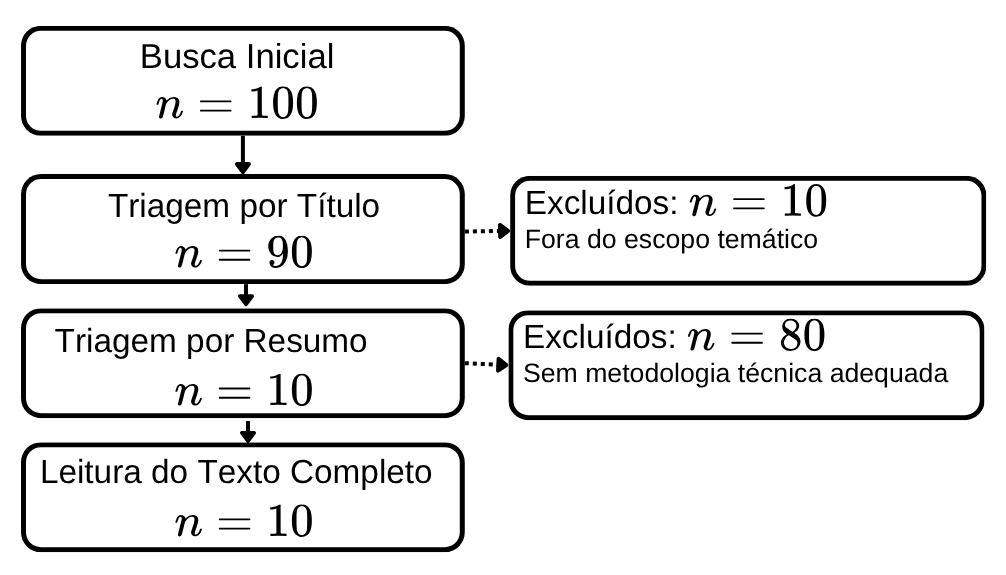
\includegraphics[width=0.65\textwidth]{./figuras/funil-pesquisa.png} 
    \caption{Funil metodológico da seleção e filtragem da pesquisa bibliográfica.}
    \label{fig:funil_pesquisa}
    \source{Autoria própria (2026).}
\end{figure}
 
% ---------------------------------------------------------------
\section{Fundamentos teóricos}
\label{sec:fundamentos}

Este capítulo apresenta os principais fundamentos teóricos e tecnológicos que sustentam o desenvolvimento do sistema proposto. Inicialmente, estabelece-se o panorama através dos conceitos de Inteligência Artificial e \textit{Machine Learning}, delimitando o paradigma computacional adotado. Em seguida, são abordados os conceitos de visão computacional, MediaPipe e \textit{landmarks}, responsáveis pela captura e representação dos sinais em Libras. Posteriormente, detalha-se o universo do \textit{Deep Learning}, incluindo o funcionamento de redes CNN e redes LSTM, aplicadas no reconhecimento de sinais estáticos e dinâmicos. Por fim, são discutidos os conceitos de Processamento de Linguagem Natural (NLP), as árvores de dependência sintática, os Modelos de Linguagem de Grande Escala (LLM) e as métricas de avaliação empregadas no sistema.

\subsection{Língua Brasileira de Sinais (Libras)}

De acordo com a \citeonline{Brasil2005}, Língua Brasileira de Sinais (Libras) é uma língua natural, completa e autônoma, utilizada pela comunidade surda no Brasil, reconhecida pela Lei nº 10.436/2002 e regulamentada pelo Decreto nº 5.626/2005 como meio legal de comunicação e expressão. Possui estrutura gramatical própria, independente da Língua Portuguesa, e está inserida em um contexto cultural e linguístico específico da comunidade surda.

O reconhecimento legal da Libras não ocorreu de forma isolada, mas como parte de um processo gradual de consolidação de direitos linguísticos e de acessibilidade para a comunidade surda, que se estende por mais de uma década. A Figura \ref{fig:linha_tempo_libras} sintetiza os principais marcos dessa trajetória legislativa, desde o reconhecimento da Libras como meio legal de comunicação, em 2002, até o fortalecimento das políticas de acessibilidade previstas na Lei Brasileira de Inclusão da Pessoa com Deficiência, em 2015.
 
\begin{figure}[htbp]
\centering
\caption{Linha do tempo da legislação brasileira sobre a Libras.}
\label{fig:linha_tempo_libras}
\begin{tikzpicture}[
  every node/.style={font=\footnotesize},
  dot/.style={circle, fill=black, minimum size=4pt, inner sep=0pt}
]
  % Eixo principal
  \draw[thick, -{Stealth}] (0,0) -- (13,0);
 
  % 2002 - acima
  \node[dot] (d1) at (1.5,0) {};
  \draw (d1) -- ++(0,0.5);
  \node[font=\bfseries\small] at (1.5,0.75) {2002};
  \node[align=center, text width=3.1cm] at (1.5,1.9) {Lei n\textordmasculine{} 10.436\\[2pt]Reconhece a Libras como meio legal de comunicação e expressão};
 
  % 2005 - abaixo
  \node[dot] (d2) at (5,0) {};
  \draw (d2) -- ++(0,-0.5);
  \node[font=\bfseries\small] at (5,-0.75) {2005};
  \node[align=center, text width=3.1cm] at (5,-1.9) {Decreto n\textordmasculine{} 5.626\\[2pt]Regulamenta a Lei 10.436; institui a Libras como disciplina curricular};
 
  % 2010 - acima
  \node[dot] (d3) at (8.5,0) {};
  \draw (d3) -- ++(0,0.5);
  \node[font=\bfseries\small] at (8.5,0.75) {2010};
  \node[align=center, text width=3.1cm] at (8.5,1.9) {Lei n\textordmasculine{} 12.319\\[2pt]Regulamenta a profissão de tradutor e intérprete de Libras};
 
  % 2015 - abaixo
  \node[dot] (d4) at (12,0) {};
  \draw (d4) -- ++(0,-0.5);
  \node[font=\bfseries\small] at (12,-0.75) {2015};
  \node[align=center, text width=3.1cm] at (12,-1.9) {Lei n\textordmasculine{} 13.146 (LBI)\\[2pt]Reforça a acessibilidade e o uso da Libras em diferentes contextos};
\end{tikzpicture}
\noindent\footnotesize{\newline \textbf{Fonte:} Elaborado pelos autores com base em \citeonline{Brasil2002}, \citeonline{Brasil2005}, \citeonline{Brasil2010} e \citeonline{Brasil2015}.}
\end{figure}

A Lei nº 10.436/2002 foi o marco inicial desse processo. Antes de sua promulgação, a Libras não possuía qualquer status legal no Brasil, o que contribuía para a invisibilidade da língua e para a marginalização de seus usuários em contextos escolares, de saúde e de serviços públicos. 

A lei é sucinta, mas simbolicamente decisiva: reconhece a Libras como meio legal de comunicação e expressão da comunidade surda brasileira, determina que o poder público deve apoiar seu uso e difusão, e prevê que sistemas educacionais devam garantir formas de apoiar seu ensino. 

É importante destacar que a própria lei ressalva que a Libras não substitui a modalidade escrita da Língua Portuguesa, ou seja, o objetivo não é sobrepor uma língua à outra, mas garantir a coexistência de ambas na vida da pessoa surda.
 
O Decreto nº 5.626/2005 surgiu justamente para dar efetividade prática à Lei nº 10.436/2002, que, por si só, não estabelecia mecanismos concretos de implementação. O decreto foi responsável por tornar a Libras disciplina curricular obrigatória nos cursos de licenciatura e nos cursos de Fonoaudiologia em todo o país, estabelecendo prazos e percentuais mínimos de adesão das instituições de ensino.

Além disso, criou critérios para a formação e certificação de professores, instrutores e tradutores/intérpretes de Libras, inclusive por meio de exames de proficiência (Prolibras), e assegurou o direito à educação bilíngue para pessoas surdas, com a Libras como primeira língua e o português escrito como segunda língua. 

Em outras palavras, o decreto transformou o reconhecimento simbólico de 2002 em obrigações concretas para as instituições de ensino, sendo considerado um divisor de águas para a formação de profissionais qualificados em Libras no Brasil.
 
A Lei nº 12.319/2010 avançou em uma frente diferente: a profissionalização do intérprete. Até então, a atuação de tradutores e intérpretes de Libras carecia de regulamentação formal, o que dificultava o reconhecimento da categoria e a garantia de padrões mínimos de qualificação e conduta ética. 

A lei define as competências do tradutor e intérprete de Libras, os requisitos mínimos de formação (nível médio ou superior, complementados por exame de proficiência), e as atribuições do profissional, que vão desde a interpretação em salas de aula e concursos públicos até o apoio em depoimentos judiciais. 

Também estabelece princípios éticos de atuação, como imparcialidade, sigilo e respeito à cultura surda. Essa regulamentação foi fundamental para consolidar o intérprete de Libras como uma carreira reconhecida, ampliando a oferta de profissionais qualificados nos mais diversos contextos sociais.
 
Por fim, a Lei nº 13.146/2015, conhecida como Lei Brasileira de Inclusão da Pessoa com Deficiência (LBI) ou Estatuto da Pessoa com Deficiência, inspirada na Convenção sobre os Direitos das Pessoas com Deficiência da ONU, não trata exclusivamente da Libras, mas insere a língua em um arcabouço mais amplo de direitos à acessibilidade comunicacional. 

A LBI reforça, entre outros pontos, o direito à educação bilíngue, a obrigatoriedade de intérpretes de Libras em instituições de ensino superior, a disponibilização de recursos de acessibilidade em serviços de saúde, eventos culturais e científicos, e a formação continuada de tradutores e intérpretes pelo poder público. 

Ao consolidar, em uma única lei nacional, direitos que antes estavam dispersos em normas variadas, a LBI ampliou a exigibilidade da Libras como direito de acessibilidade em praticamente todas as esferas da vida social.

Do ponto de vista linguístico, a Libras pertence à modalidade visual-espacial, caracterizando-se pela capacidade de expressar múltiplos blocos de informação simultaneamente por meio da combinação de sinais, movimentos e expressões faciais. Esse modelo contrapõe-se diretamente à modalidade oral-auditiva da língua portuguesa, cuja estrutura é essencialmente linear e baseada na organização de elementos em uma sequência fonética e temporal fixa.

As expressões faciais e corporais possuem papel fundamental na Libras, não sendo utilizadas apenas para transmitir emoções, mas também como elementos gramaticais da língua. Conhecidas como Expressões Não Manuais (ENM), elas complementam os sinais realizados com as mãos e auxiliam na construção do significado das frases \cite{Quadros2004}. Em muitos casos, a ausência dessas expressões pode dificultar a compreensão ou até alterar o sentido do enunciado.

Diferentes movimentos do rosto podem indicar intenções comunicativas específicas. Expressões faciais associadas ao movimento das sobrancelhas, por exemplo, podem marcar perguntas, negações e intensificações, funcionando como elementos linguísticos da estrutura da Libras \cite{Brito1995}. Além disso, movimentos da boca, direção do olhar e expressões corporais também contribuem para a construção da mensagem e para a fluidez da comunicação.

No nível fonológico, os sinais são formados por parâmetros básicos, conforme detalhado na Figura~\ref{fig:sinais}: a configuração de mão (CM), o movimento (M), a locação (L), a orientação (Or) e as expressões não manuais (ENM). A combinação desses elementos forma os sinais, e mudanças em qualquer um desses parâmetros podem alterar o significado.

\begin{figure}[H]
    \centering
    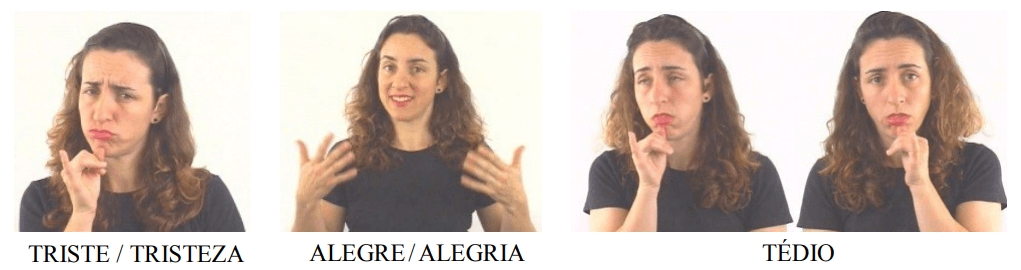
\includegraphics[width=0.8\textwidth]{./figuras/sinaisLibras.png}
    \caption{Parâmetros de formação do sinal na Libras.}
    \label{fig:sinais}
    \fonte{\citeonline{Felipe2013}.}
\end{figure}

Estudos mostram que as línguas de sinais possuem as mesmas propriedades das línguas naturais, como criatividade, organização por regras e capacidade de expressar qualquer tipo de conteúdo \cite{Quadros2004}.

Do ponto de vista morfológico, a Libras apresenta uma estrutura diferente da língua portuguesa. Em vez de adicionar partes de forma sequencial (como prefixos e sufixos), os elementos do sinal são combinados ao mesmo tempo. Por exemplo, informações como número, negação e até mesmo o objeto da ação podem ser incorporadas diretamente ao sinal. Além disso, a relação entre o sujeito e o objeto da ação pode ser indicada pela direcionalidade do movimento, que conecta os pontos de referência criados durante a comunicação.

No nível sintático, a língua portuguesa segue predominantemente a ordem Sujeito-Verbo-Objeto (SVO). Já a Libras apresenta maior flexibilidade, sendo possíveis diferentes organizações, como SVO, SOV, OSV e VOS, dependendo do contexto. Isso ocorre porque a língua utiliza o espaço para indicar relações entre os elementos da frase, reduzindo a necessidade de uma ordem fixa.

Para demonstrar a flexibilidade sintática da Libras e como ela contrasta com a estrutura linear do português, considera-se a sentença composta pelos tokens sinalizados \texttt{[VOCÊ, QUERER, ÁGUA]} \cite{Lopez2017}. Enquanto na língua portuguesa o enunciado possui uma organização predominantemente fixa, na Libras a ordem varia conforme o foco e o contexto comunicativo \cite{Quadros2004}. 

A Tabela \ref{tab:variacoes_libras} ilustra como o pipeline de Processamento de Linguagem Natural (NLP) mapeia os componentes de Sujeito (S), Verbo (V) e Objeto (O) sob quatro tipologias frasais distintas, executando a função de reordenação $\pi$ necessária para convergir na estrutura alvo unificada do português.

\begin{table}[H]
\centering
\caption{Mapeamento estrutural das variações frasais da Libras para o Português (SVO).}
\label{tab:variacoes_libras}
\small
\begin{tabularx}{\textwidth}{lXll}
\hline
\textbf{Tipologia} & \textbf{Sequência de Tokens (Libras)} & \textbf{Componentes}  \\ \hline
\textbf{SVO}       & [VOCÊ] [QUERER] [ÁGUA]                & Sujeito + Verbo + Objeto           \\
\textbf{SOV}       & [VOCÊ] [ÁGUA] [QUERER]                & Sujeito + Objeto + Verbo            \\
\textbf{OSV}       & [ÁGUA] [VOCÊ] [QUERER]                & Objeto + Sujeito + Verbo           \\
\textbf{VOS}       & [QUERER] [ÁGUA] [VOCÊ]                & Verbo + Objeto + Sujeito            \\ \hline
\end{tabularx}
\noindent\footnotesize{\newline \textbf{Fonte:} Autoria própria (2026), baseado em \citeonline{Quadros2004} e \citeonline{Jurafsky2023}.}
\end{table}

Essas diferenças impactam diretamente o processo de tradução. Elementos comuns no português, como artigos e preposições, nem sempre aparecem de forma explícita na Libras, pois muitas dessas relações são expressas pelo uso do espaço e pelo contexto. Por isso, sistemas computacionais precisam não apenas reconhecer os sinais, mas também reorganizar as informações e incluir elementos necessários para gerar frases corretas em português.


\subsection{Inteligência Artificial}

A Inteligência Artificial (IA) é um campo da Ciência da Computação dedicado ao desenvolvimento de sistemas capazes de executar tarefas que normalmente requerem inteligência humana, como percepção, raciocínio, aprendizado e tomada de decisão \cite{russell2021}. Seu objetivo é criar métodos computacionais capazes de interpretar informações do ambiente, extrair conhecimento a partir de dados e agir de forma autônoma para alcançar determinados objetivos.

Antigamente, os sistemas de Inteligência Artificial não aprendiam sozinhos: eles apenas seguiam regras e instruções fixas criadas e programadas por humanos. Com o aumento da disponibilidade de dados e do poder computacional, surgiram técnicas capazes de aprender padrões diretamente a partir de exemplos, consolidando o paradigma conhecido como \textit{Machine Learning} \cite{ibm_ml2026}.

O campo da Inteligência Artificial teve sua origem formalmente estabelecida na década de 1950, quando pesquisadores reunidos na Conferência de Dartmouth propuseram investigar se máquinas poderiam simular aspectos da inteligência humana \cite{russell2021}. 

Nas décadas seguintes, o desenvolvimento da área alternou períodos de grande investimento e otimismo com fases de estagnação, conhecidas como invernos da Inteligência Artificial, motivadas principalmente pelas limitações computacionais da época e pela dificuldade de generalização dos sistemas baseados exclusivamente em regras fixas. 

Apenas com o avanço do poder de processamento, a disponibilidade de grandes volumes de dados e o aperfeiçoamento das técnicas de aprendizado profundo a área retomou um crescimento consistente, culminando nas aplicações observadas atualmente \cite{russell2021}.

Atualmente, a Inteligência Artificial engloba diversas áreas de pesquisa e aplicação, incluindo \textit{machine learning}, visão computacional, processamento de linguagem natural, robótica e sistemas de recomendação. Essas áreas compartilham o objetivo comum de permitir que sistemas computacionais interpretem informações complexas e realizem tarefas que anteriormente dependiam exclusivamente da capacidade humana \cite{russell2021}.
Quanto ao escopo de atuação, os sistemas de Inteligência Artificial podem ser classificados em Inteligência Artificial Estreita (\textit{Narrow AI}) e Inteligência Artificial Geral (\textit{General AI}). 

A primeira categoria refere-se a sistemas projetados para executar uma tarefa específica, como reconhecimento de imagens ou tradução automática, sem possuir capacidade de generalização para domínios distintos daquele para o qual foram treinados. A segunda categoria, ainda hipotética, corresponderia a sistemas capazes de replicar a versatilidade cognitiva humana em qualquer domínio de conhecimento \cite{russell2021}. 

O sistema proposto neste trabalho enquadra-se na categoria de Inteligência Artificial Estreita, uma vez que seu escopo está delimitado ao reconhecimento e à tradução de sinais em Libras para a língua portuguesa.

\subsection{Machine Learning}

O aprendizado de máquina (\textit{machine learning}) é uma subárea da Inteligência Artificial dedicada ao desenvolvimento de algoritmos capazes de aprender padrões a partir de dados e utilizá-los para realizar previsões, classificações ou tomadas de decisão sem que todas as regras precisem ser explicitamente programadas \cite{mitchell1997, faceli2021}. Em vez de depender exclusivamente de instruções definidas por um programador, os modelos ajustam seus parâmetros com base em exemplos durante o processo de treinamento.

Os métodos de \textit{machine learning} são tradicionalmente classificados em três categorias principais \cite{geron2022, oracle_machine_learning}:

\begin{itemize}
    \item Aprendizado Supervisionado: utiliza conjuntos de dados rotulados, nos quais cada exemplo de entrada está associado a uma saída esperada. O objetivo é aprender uma função capaz de realizar previsões corretas para novos dados;
    \item Aprendizado Não Supervisionado: trabalha com dados sem rótulos, buscando identificar padrões, agrupamentos ou estruturas ocultas presentes nas informações analisadas;
    \item Aprendizado por Reforço: baseia-se na interação entre um agente e um ambiente, onde o aprendizado ocorre por meio de recompensas e penalidades associadas às ações executadas.
\end{itemize}

O avanço do \textit{machine learning} impulsionou o desenvolvimento de aplicações em diversas áreas, incluindo reconhecimento de imagens, processamento de linguagem natural, sistemas de recomendação e análise preditiva \cite{faceli2021}. Entre suas vertentes, destaca-se o \textit{Deep Learning}, que utiliza redes neurais com múltiplas camadas para modelar problemas complexos a partir de grandes volumes de dados.

No contexto deste trabalho, o \textit{machine learning} fornece a base para o treinamento dos modelos responsáveis pelo reconhecimento dos sinais da Libras. A partir de exemplos previamente rotulados, os algoritmos aprendem a associar padrões extraídos dos \textit{landmarks} das mãos e do rosto às respectivas classes de sinais, possibilitando a identificação automática dos gestos realizados pelo usuário.


\subsection{Visão Computacional}

A Visão Computacional é o campo da ciência da computação que capacita máquinas a extrair informações significativas de imagens e vídeos, interpretando o meio visual de forma análoga à percepção humana \cite{Milano2014}. Segundo \citeonline{IBM2025}, enquanto a visão humana é intuitiva e imediata, as máquinas dependem de algoritmos capazes de converter pixels e dados brutos em representações estruturadas e semanticamente compreensíveis.
 
No contexto deste projeto, a visão computacional constitui a primeira e mais crítica etapa do pipeline de tradução, pois é responsável por transformar o fluxo de vídeo capturado pela câmera em vetores de características numéricas que alimentam os modelos de reconhecimento. Essa transformação ocorre em quatro etapas sequenciais, descritas a seguir e sintetizadas na Figura~\ref{fig:pipeline_vc}.
 
\begin{enumerate}
    \item A primeira etapa é a captura de \textit{frames}, em que o vídeo proveniente da webcam é segmentado em quadros individuais para processamento em tempo real. 
    \item A segunda etapa é a detecção de mãos e rosto, na qual o \textit{framework} MediaPipe analisa cada \textit{frame} para localizar e isolar as regiões de interesse, os membros superiores e a face, do restante da cena. De acordo com \citeonline{Neves2012}, essa etapa é fundamental para garantir que o sistema concentre a análise exclusivamente nas regiões que carregam informação linguística. 
    \item A terceira etapa é a extração de \textit{landmarks}, em que o MediaPipe mapeia as coordenadas tridimensionais ($x$, $y$, $z$) dos 21 pontos articulares de cada mão e dos 468 pontos-chave do rosto, produzindo uma representação geométrica compacta e invariante a variações de iluminação e tom de pele \cite{Zhang2020}. 
    \item A quarta etapa é a classificação do sinal, na qual os vetores de \textit{landmarks} são encaminhados ao módulo de aprendizado profundo: sinais estáticos são processados pela CNN, que analisa a configuração espacial da mão em um único \textit{frame}, enquanto sinais dinâmicos são processados pela LSTM, que modela a sequência temporal de \textit{landmarks} ao longo do movimento. Conforme explicam \citeonline{Pinho2004}, é justamente essa capacidade de distinguir configurações estáticas de padrões de movimento que permite identificar os diferentes elementos do léxico da Libras.
\end{enumerate}

\begin{figure}[H]
    \centering
    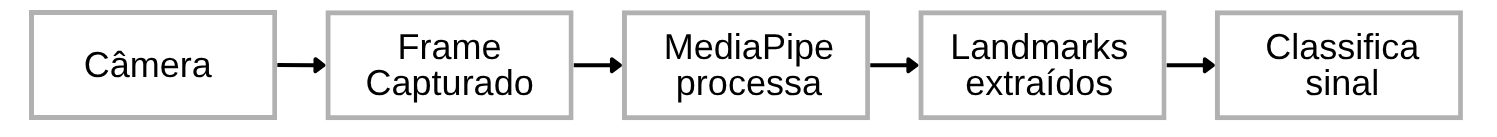
\includegraphics[width=1.0\textwidth]{./figuras/pipeline-vc.png}
    \caption{Pipeline da Visão Computacional.}
    \label{fig:pipeline_vc}
    \source{Autoria própria (2026).}
\end{figure}

\subsection{Datasets}

No desenvolvimento de modelos de \textit{Deep Learning}, o \textit{dataset} (base de dados) constitui o pilar fundamental para o treinamento e a validação do sistema. Segundo \citeonline{Schmidhuber2014}, a eficácia de arquiteturas complexas como CNNs e LSTMs depende diretamente da disponibilidade de grandes volumes de dados rotulados, que permitem ao modelo aprender representações estatísticas precisas e generalizáveis.

No contexto do reconhecimento de Libras, os \textit{datasets} apresentam desafios devido à natureza multimodal da língua. Um \textit{dataset} robusto para este fim deve conter não apenas imagens isoladas, mas sequências de vídeo que capturem a dinâmica dos sinais. De acordo com \citeonline{Silva2017}, a diversidade dos dados é crucial para mitigar problemas de overfitting, ou seja, a perda de capacidade de generalização do sistema por memorização exaustiva dos dados de treinamento, garantindo que o sistema seja capaz de reconhecer gestos realizados por diferentes usuários, com variações em:

\begin{itemize}
    \item {Antropometria:} Diferenças no tamanho, cor, formato das mãos e traços faciais dos sinalizadores;
    \item {Condições Ambientais:} Variações de iluminação e fundos de imagem (backgrounds) complexos, que testam a capacidade de segmentação do modelo;
    \item {Execução do Sinal:} Diferenças na velocidade, amplitude e fluidez do movimento, que impactam diretamente a análise temporal das redes LSTM.
\end{itemize}

Os três \textit{datasets} adotados neste projeto apresentam diversidade de dados a esse respeito: o MINDS-Libras conta com distribuição controlada, são 6 pessoas realizando 5 repetições de cada um dos 20 sinais, resultando em classes uniformes \cite{Rezende2021}; o V-Librasil possui estrutura regular, com 3 gravações por sinal para cada um dos 1.364 termos \cite{Rodrigues2021}; já o \textit{dataset} \textit{Libras Brazilian Sign Language}, composto por imagens estáticas do alfabeto manual, apresenta variação no número de amostras entre as classes, característica comum em \textit{datasets} tratados a partir de fontes variadas \cite{Pas2020}. 

Além disso, a estruturação do \textit{dataset} deve prever a divisão entre conjuntos de treinamento, validação e teste. Conforme explicam \citeonline{Goodfellow2016}, essa separação é o que permite avaliar a capacidade de generalização do algoritmo frente a dados nunca vistos, assegurando que o tradutor de Libras funcione corretamente em cenários do mundo real e não apenas em ambientes controlados de laboratório.

\subsection{Pré-processamento de Dados}

Antes da aplicação dos modelos de \textit{deep learning}, é necessária uma etapa de pré-processamento dos dados visuais, com o objetivo de melhorar a qualidade das informações fornecidas ao sistema e aumentar a precisão do reconhecimento dos sinais.

O pré-processamento envolve técnicas de tratamento de imagem, como redimensionamento dos \textit{frames}, normalização dos valores de pixel e remoção de ruídos. Além disso, podem ser aplicados filtros para suavização da imagem e ajuste de contraste, reduzindo interferências causadas por variações de iluminação e fundo. Segundo \citeonline{Szeliski2010}, essas etapas são fundamentais para garantir que os algoritmos de visão computacional consigam extrair características relevantes de forma eficiente. 

Para ampliar a diversidade do conjunto de treinamento e reduzir problemas de \textit{overfitting}, será aplicado \textit{data augmentation} sobre os dados visuais, por meio de operações como espelhamento, rotações e variações de velocidade dos vídeos \cite{Goodfellow2016}, conforme ilustrado na Figura \ref{fig:data_augmentation}. Essas transformações aumentam artificialmente a diversidade do conjunto de treinamento, melhorando a capacidade de generalização dos modelos.

\begin{figure}[H]
    \centering
    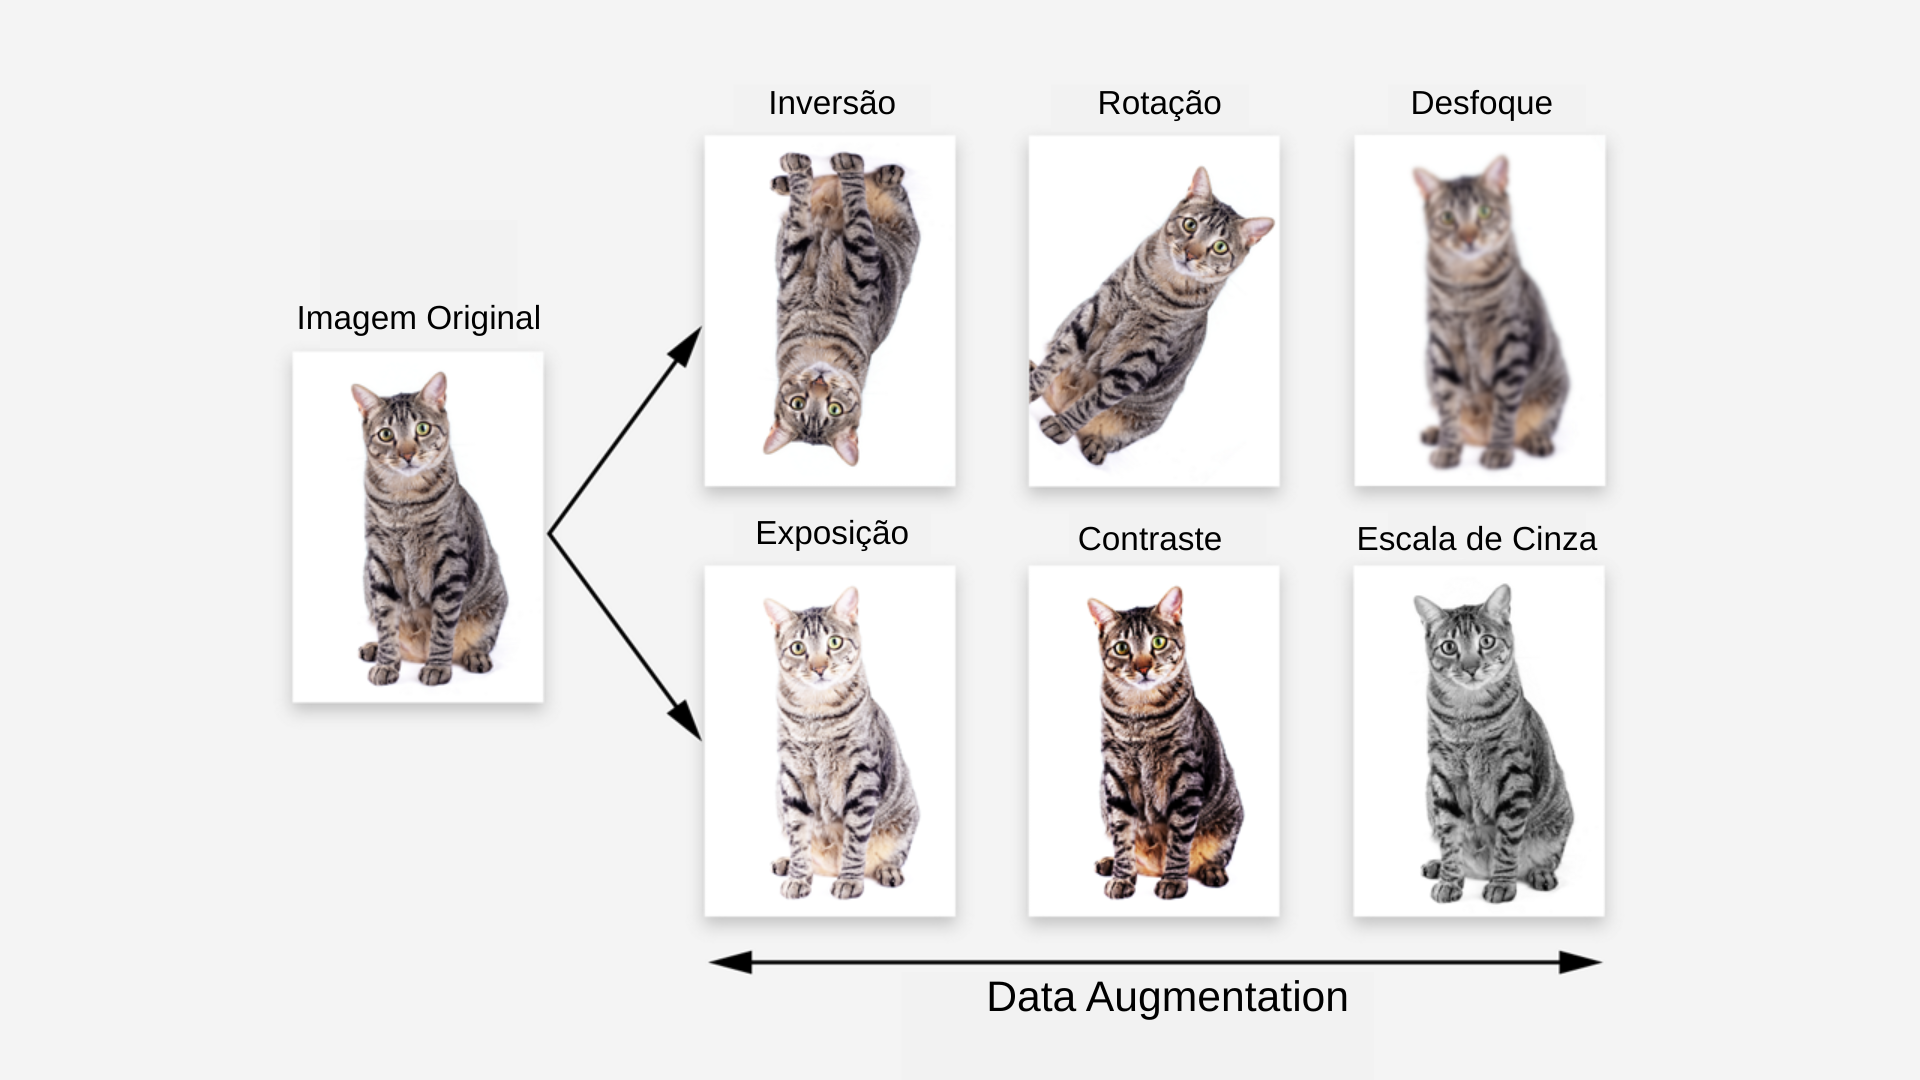
\includegraphics[width=1.0\textwidth]{./figuras/data-augmentation-image-augment.png}
    \caption{Exemplo de técnicas de \textit{Data Augmentation}.}
    \label{fig:data_augmentation}
    \noindent\footnotesize{Fonte: Adaptado \citeonline{murel2024data}.}
\end{figure}

Outro aspecto relevante é a padronização dos dados de entrada, garantindo que todas as imagens ou sequências possuam dimensões e formatos consistentes. Essa uniformidade é essencial para funcionamento correto das redes neurais, especialmente em modelos baseados em CNN e LSTM.

Também é importante o balanceamento de classes. Em \textit{datasets} de reconhecimento de sinais, é comum que determinadas classes possuam um número de amostras significativamente maior do que outras. Quando treinado sobre dados desbalanceados, o modelo tende a favorecer as classes com maior quantidade, comprometendo o desempenho nas classes com menor representatividade \cite{Chawla2002}. Para mitigar esse efeito, será adotada a ponderação de classes na função de perda durante o treinamento, penalizando mais os erros cometidos nas classes menos frequentes \cite{Goodfellow2016}.

Para consolidar a regularização estatística do pipeline, aplica-se a técnica SMOTE (\textit{Synthetic Minority Over-sampling Technique}) sobre os vetores de \textit{landmarks} extraídos pelo MediaPipe, gerando exemplos sintéticos por interpolação matemática entre amostras próximas no espaço de características, sem manipular diretamente os pixels brutos \cite{Chawla2002}. Por fim, os dados serão divididos em conjuntos de treinamento, validação e teste, separação que, conforme explicam \citeonline{Goodfellow2016}, é o que permite avaliar a capacidade de generalização do modelo frente a dados nunca vistos, assegurando que o tradutor funcione corretamente em cenários reais e não apenas em ambientes controlados de laboratório.

\subsection{MediaPipe \& Landmarks}

O \textit{MediaPipe} é um \textit{framework} de código aberto desenvolvido pelo Google para a construção de pipelines de percepção multimodal em tempo real \cite{Lugaresi2019}. Ele disponibiliza soluções pré-treinadas para tarefas de visão computacional, incluindo detecção de pose corporal, rastreamento de mãos e rastreamento facial. No contexto deste trabalho, destacam-se os módulos \textit{MediaPipe Hands} e \textit{MediaPipe Face Mesh}, utilizados para extrair os \textit{landmarks} das mãos e do rosto que servirão como entrada para os modelos de reconhecimento dos sinais da Libras.

Os \textit{landmarks}, ou pontos-chave, são as coordenadas tridimensionais (x,y,z) extraídas por essas soluções de partes anatomicamente relevantes do corpo, articulações das mãos e regiões do rosto, utilizadas para representar a geometria e o movimento dos sinais de forma compacta e independente de variações de iluminação ou tom de pele \cite{Zhang2020}.

A solução \textit{MediaPipe Hands} opera em dois estágios sequenciais \cite{Zhang2020}. No primeiro, um detector leve baseado em \textit{deep learning} localiza a palma da mão na imagem completa, produzindo um \textit{bounding box} delimitador. No segundo, um modelo de regressão de \textit{landmarks} recebe o recorte da mão e estima as coordenadas tridimensionais ($x$, $y$, $z$) de 21 pontos-chave que representam as articulações dos dedos e o pulso, conforme ilustrado na Figura~\ref{fig:mediapipe}. As coordenadas $x$ e $y$ são normalizadas em relação às dimensões do \textit{frame} (valores entre 0 e 1), enquanto $z$ representa a profundidade relativa ao pulso, permitindo inferir a orientação tridimensional da mão mesmo com uma câmera \cite{Zhang2020}.

\begin{figure}[H]
    \centering
    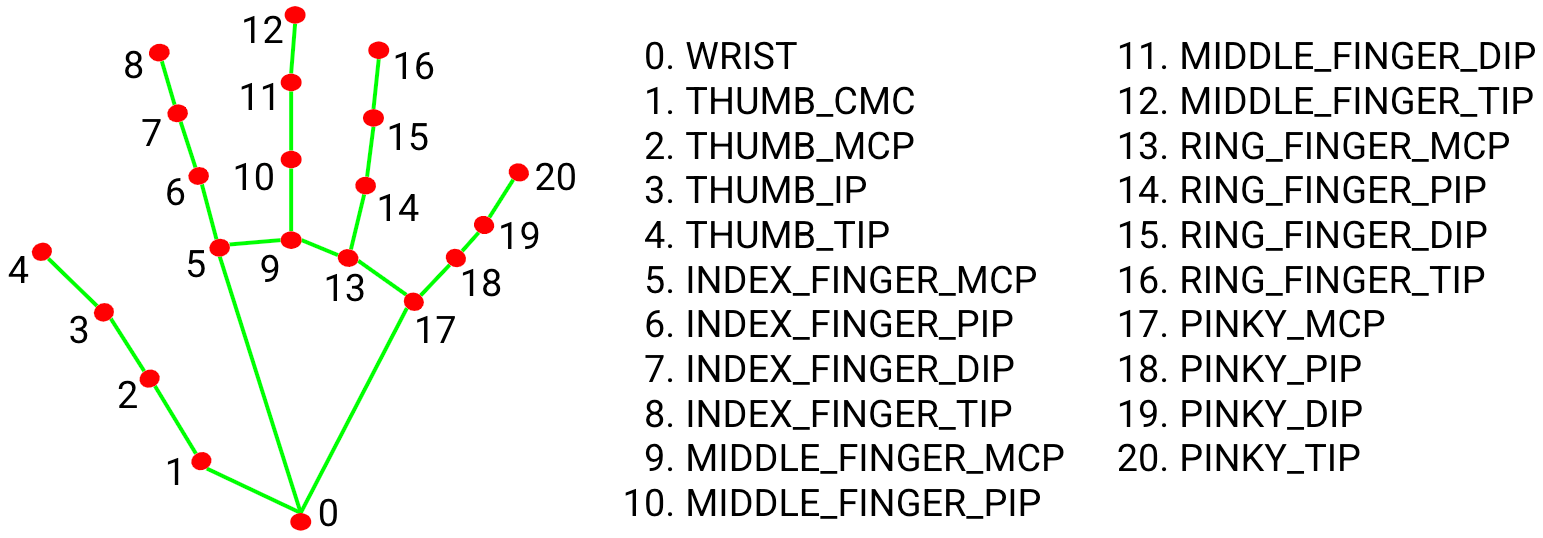
\includegraphics[width=0.8\textwidth]{./figuras/hand_landmarks.png}
    \caption{Esquema dos 21 \textit{landmarks} detectados pelo \textit{MediaPipe Hands}.}
    \label{fig:mediapipe}
    \fonte{\citeonline{tensorflow2021hand}.} 
\end{figure}

O \textit{MediaPipe Face Mesh}, por sua vez, mapeia 468 pontos-chave do rosto em tempo de execução, distribuídos pelas regiões de sobrancelha, olhos, bochecha e boca, conforme ilustrado na Figura~\ref{fig:facemesh} \cite{Lugaresi2019}. Essa cobertura é essencial para a captura das Expressões Não Manuais (ENM) da Libras, como a elevação de sobrancelhas para marcação de perguntas e a contração facial para negação, que exercem função gramatical obrigatória na língua e não podem ser ignoradas sem perda de significado \cite{Brito1995}.

\begin{figure}[H]
    \centering
    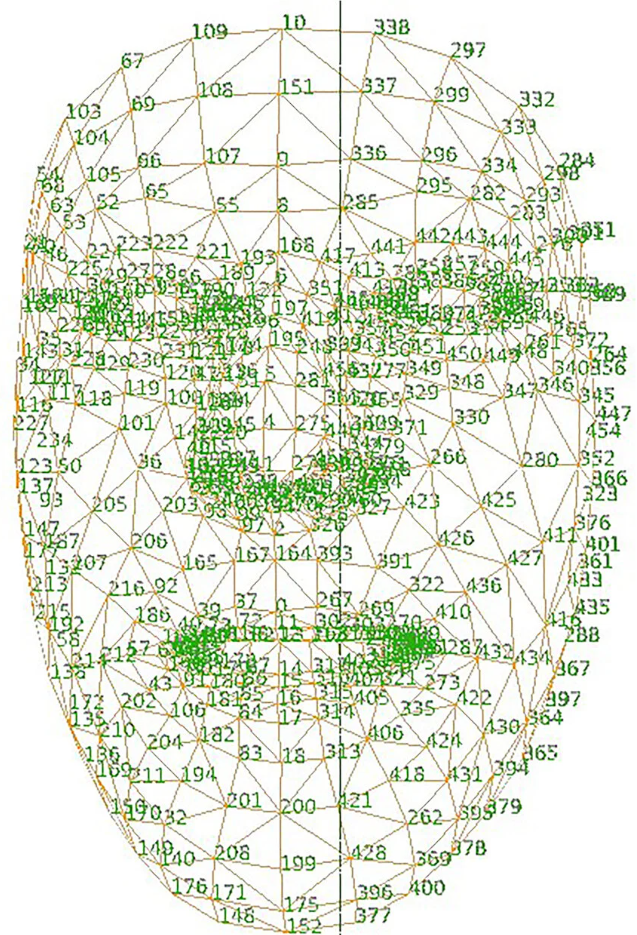
\includegraphics[width=0.4\textwidth]{./figuras/facemesh_landmarks.png}
    \caption{Esquema dos 468 \textit{landmarks} detectados pelo \textit{MediaPipe Face Mesh}.}
    \label{fig:facemesh}
    \fonte{\citeonline{Khaleeletal2024}.} 
\end{figure}

No contexto deste projeto, os dois módulos operam simultaneamente sobre o mesmo \textit{frame}, fornecendo ao sistema um vetor de entrada combinado que representa tanto a configuração manual quanto a expressão facial do sinalizador. Essa representação é invariante a variações de aparência física entre usuários, pois baseia-se em geometria articular e não em pixels brutos, reduzindo drasticamente a dimensionalidade dos dados e tornando o treinamento mais eficiente e generalizável \cite{Lugaresi2019}.

\subsection{Deep Learning}

O \textit{Deep Learning}, ou Aprendizado Profundo, é uma subárea do \textit{Machine Learning} que utiliza redes neurais artificiais com múltiplas camadas de processamento. Segundo a \citeonline{IBM2026}, essa abordagem é inspirada na estrutura do cérebro humano, onde cada camada de "neurônios"\ executa operações matemáticas para aprender representações cada vez mais abstratas dos dados.

Diferente dos métodos tradicionais, o \textit{deep learning} permite que o sistema identifique características automaticamente, sem a necessidade de intervenção humana manual. Conforme explica a \citeonline{Oracle2022}, essa capacidade de autoajuste através de pesos e vieses é o que torna os modelos extremamente precisos para resolver problemas complexos.

No nível matemático, cada camada de uma rede neural profunda executa uma transformação sobre o vetor de entrada recebido da camada anterior. Formalmente, para uma camada $l$, essa transformação é definida como:

\begin{equation}
    \mathbf{a}^{(l)} = f\!\left(\mathbf{W}^{(l)}\,\mathbf{a}^{(l-1)} + \mathbf{b}^{(l)}\right)
    \label{eq:forward}
\end{equation}

\noindent onde $\mathbf{a}^{(l)}$ é o vetor de ativações da camada $l$, $\mathbf{W}^{(l)}$ é a matriz de pesos, $\mathbf{b}^{(l)}$ é o vetor de vieses e $f(\cdot)$ é a função de ativação, responsável por introduzir não-linearidade ao modelo. Entre as funções de ativação mais utilizadas está a ReLU (\textit{Rectified Linear Unit}), definida como $f(x) = \max(0, x)$, que suprime ativações negativas e acelera a convergência do treinamento \cite{Goodfellow2016}.

Para que a rede aprenda, é necessário quantificar o erro entre a saída prevista $\hat{y}$ e o valor real $y$ por meio de uma função de perda $\mathcal{L}$. No caso de classificação multiclasse, utiliza-se tipicamente a entropia cruzada:

\begin{equation}
    \mathcal{L} = -\sum_{c=1}^{C} y_c \log\hat{y}_c
    \label{eq:loss}
\end{equation}

\noindent onde $C$ é o número de classes e $y_c$ indica se a amostra pertence à classe $c$. A minimização de $\mathcal{L}$ é realizada pelo algoritmo de \textit{backpropagation}, que propaga o gradiente da função de perda de volta pelas camadas da rede, atualizando cada peso $w$ segundo a regra do gradiente descendente \cite{Goodfellow2016}:

\begin{equation}
    w \leftarrow w - \eta \,\frac{\partial \mathcal{L}}{\partial w}
    \label{eq:grad}
\end{equation}

\noindent onde $\eta$ é a taxa de aprendizado (\textit{learning rate}), que controla o tamanho do passo de atualização. Esse ciclo de propagação direta, cálculo da perda e retropropagação do gradiente é repetido iterativamente sobre o conjunto de treinamento até que o modelo convirja para uma configuração de pesos capaz de generalizar para dados novos \cite{Goodfellow2016}.

Um dos principais motivos para a ampla adoção desta tecnologia é o seu desempenho em tarefas que envolvem visão computacional e processamento de texto. De acordo com \citeonline{Schmidhuber2014}, o aprendizado profundo revolucionou o reconhecimento de padrões ao permitir a análise de grandes volumes de dados não estruturados.

No contexto deste projeto, o uso do \textit{deep learning} justifica-se pela necessidade de tratar informações visuais e sequenciais simultaneamente. Segundo \citeonline{Goodfellow2016}, redes profundas são aproximadores universais capazes de mapear entradas complexas para saídas específicas, como a tradução de um gesto em texto.

Dessa forma, a profundidade dessas redes permite que o sistema capture desde detalhes mínimos de um \textit{frame} até o contexto completo de uma frase em Libras. Conforme destacam \citeonline{Fleck2016}, essa estrutura multicamada é essencial para que o modelo aprenda padrões que seriam invisíveis para algoritmos de aprendizado mais simples. Uma representação visual desse fluxo de informações através de múltiplas camadas pode ser observada na Figura \ref{fig:deep_learning}.

\begin{figure}[H]
    \centering
    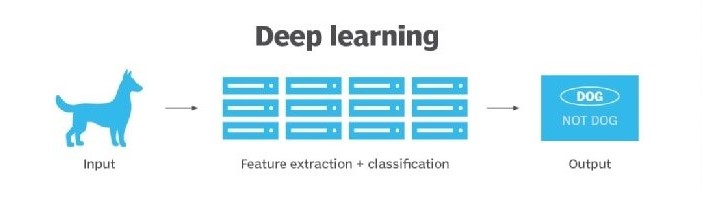
\includegraphics[width=1.0\textwidth]{./figuras/deepLearning.jpg}
    \caption{Fluxo de processamento hierárquico em uma arquitetura de Deep Learning.}
    \label{fig:deep_learning}
    \noindent\footnotesize{Fonte: \citeonline{computerweekly2026deep}.}
\end{figure}


\subsection{Redes Neurais Convolucionais}

As Redes Neurais Convolucionais (CNN) são arquiteturas de \textit{deep learning} especializadas no processamento de dados com topologia em grade, como imagens e sequências. Introduzidas por \citeonline{Lecun1998} e popularizadas com o modelo AlexNet \cite{Krizhevsky2012}, as CNNs revolucionaram o campo da visão computacional ao substituir a extração manual de características por um processo de aprendizado automático e hierárquico.

No escopo deste trabalho, a CNN é utilizada para o reconhecimento de sinais estáticos, como as configurações de mão do alfabeto manual da Libras, nos quais a identificação do sinal depende exclusivamente da configuração espacial da mão em um único \textit{frame} \cite{Fleck2016}.

A arquitetura de uma CNN é composta por três tipos principais de camadas que se alternam e se combinam ao longo da rede \cite{Goodfellow2016}:

\begin{enumerate}

  \item Camada de Convolução: Conjunto de filtros (também chamados de \textit{kernels}) de tamanho reduzido, tipicamente $3 \times 3$ ou $5 \times 5$ pixels, desliza sobre a imagem de entrada, calculando o produto escalar entre os pesos do filtro e os pixels da região coberta. Matematicamente, para uma imagem de entrada $I$ e um filtro $K$, a operação de convolução discreta é definida como:

  \begin{equation}
      (I * K)(i, j) = \sum_{m}\sum_{n} I(i+m,\; j+n) \cdot K(m, n)
  \end{equation}
  $I$: Imagem de entrada. \\
  $K$: Filtro ou \textit{kernel}. \\
  $(i, j)$: Posição atual do pixel na saída (mapa de características). \\
  $(m, n)$: Índices do \textit{kernel}. \\

  O resultado é chamado de mapa de ativação, que representa a presença de um determinado padrão visual (como bordas, curvas ou texturas) em cada posição espacial da imagem \cite{Goodfellow2016}. O compartilhamento de pesos entre todas as posições da imagem reduz drasticamente o número de parâmetros treináveis e confere à CNN invariância à translação, o modelo reconhece o padrão independentemente de onde ele aparece na imagem \cite{Fleck2016}.

  \item Camada de Pooling: Após a convolução, a camada de \textit{pooling} realiza uma subamostragem espacial dos mapas de ativação, reduzindo suas dimensões e, com isso, a quantidade de parâmetros e o custo computacional das camadas subsequentes. A operação mais comum é o Max Pooling, que seleciona o valor máximo dentro de uma janela de tamanho fixo (por exemplo, $2 \times 2$), retendo as características mais proeminentes e descartando informações redundantes \cite{Lecun1998}. Esse mecanismo também contribui para a robustez do modelo a pequenas variações de posição e escala dos objetos.

  \item Camadas Totalmente Conectadas: Ao final da rede, após um conjunto de camadas de convolução e \textit{pooling}, os mapas de ativação são linearizados e alimentados em uma ou mais camadas totalmente conectadas, que funcionam como um classificador tradicional. Nessa etapa, as representações abstratas aprendidas pelas camadas anteriores são combinadas para gerar a predição final, por exemplo, a probabilidade de que o gesto capturado corresponda a cada letra do alfabeto manual \cite{Furtado2019}.

\end{enumerate}

A integração sequencial e o fluxo de dados entre essas três camadas fundamentais que compõem a topologia da rede estão ilustrados na Figura \ref{fig:cnn_arquitetura}.

\begin{figure}[H]
    \centering
    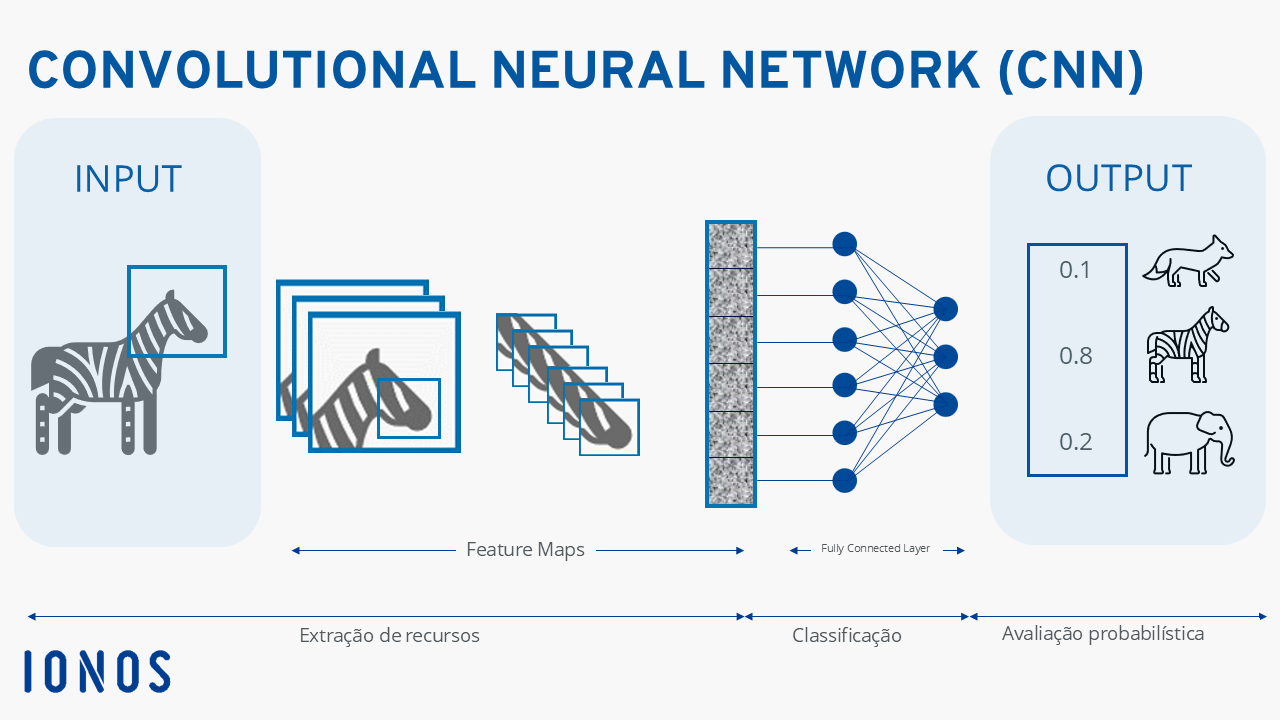
\includegraphics[width=0.9\textwidth]{./figuras/cnn.png}
    \caption{Diagrama de blocos e fluxo de dados em uma Rede Neural Convolucional.}
    \label{fig:cnn_arquitetura}
    \noindent\footnotesize{Fonte: \citeonline{ionos2026cnn}.}
\end{figure}

No contexto deste projeto, os \textit{landmarks} extraídos pelo MediaPipe (coordenadas $x$, $y$, $z$ das articulações da mão) são organizados como vetores de entrada para a CNN. A rede aprende, durante o treinamento, quais combinações de posições articulares são discriminativas para cada sinal estático. 

Conforme apontam \citeonline{Fleck2016}, o sucesso das CNNs em tarefas de visão computacional deve-se à sua capacidade de identificar características locais de forma hierárquica: as camadas iniciais capturam padrões simples (orientação dos dedos, curvatura das juntas) e as camadas mais profundas combinam esses padrões em representações de alto nível (configuração completa da mão). Essa configuração garante maior robustez a variações de iluminação e enquadramento \cite{Furtado2019}.

\subsection{Redes de Memória de Longo Prazo}

Para o reconhecimento de sinais dinâmicos em vídeo, onde o significado do gesto reside no movimento ao longo do tempo, utiliza-se a \textit{Long Short-Term Memory} (LSTM). Esta arquitetura é uma evolução das Redes Neurais Recorrentes (RNN) tradicionais, introduzida por \citeonline{Hochreiter1997} para solucionar a limitação do desaparecimento do gradiente (\textit{vanishing gradient}), que impede redes comuns de aprenderem dependências de longo prazo em sequências de dados.

O diferencial da LSTM é a sua unidade de memória interna, frequentemente chamada de célula, que permite a manutenção de informações por intervalos de tempo estendidos \cite{Hochreiter1997}. Essa estrutura é fundamental para o aprendizado de sequências complexas, como a linguagem de sinais, onde a predição ou classificação de um gesto depende de \textit{frames} ocorridos em instantes anteriores \cite{Bayer2009}.

A arquitetura da célula da LSTM, ilustrada detalhadamente na Figura \ref{fig:lstm}, é composta por três componentes principais, conhecidos como "portões" (\textit{gates}), que controlam o fluxo de informação:

\begin{figure}[H]
    \centering
    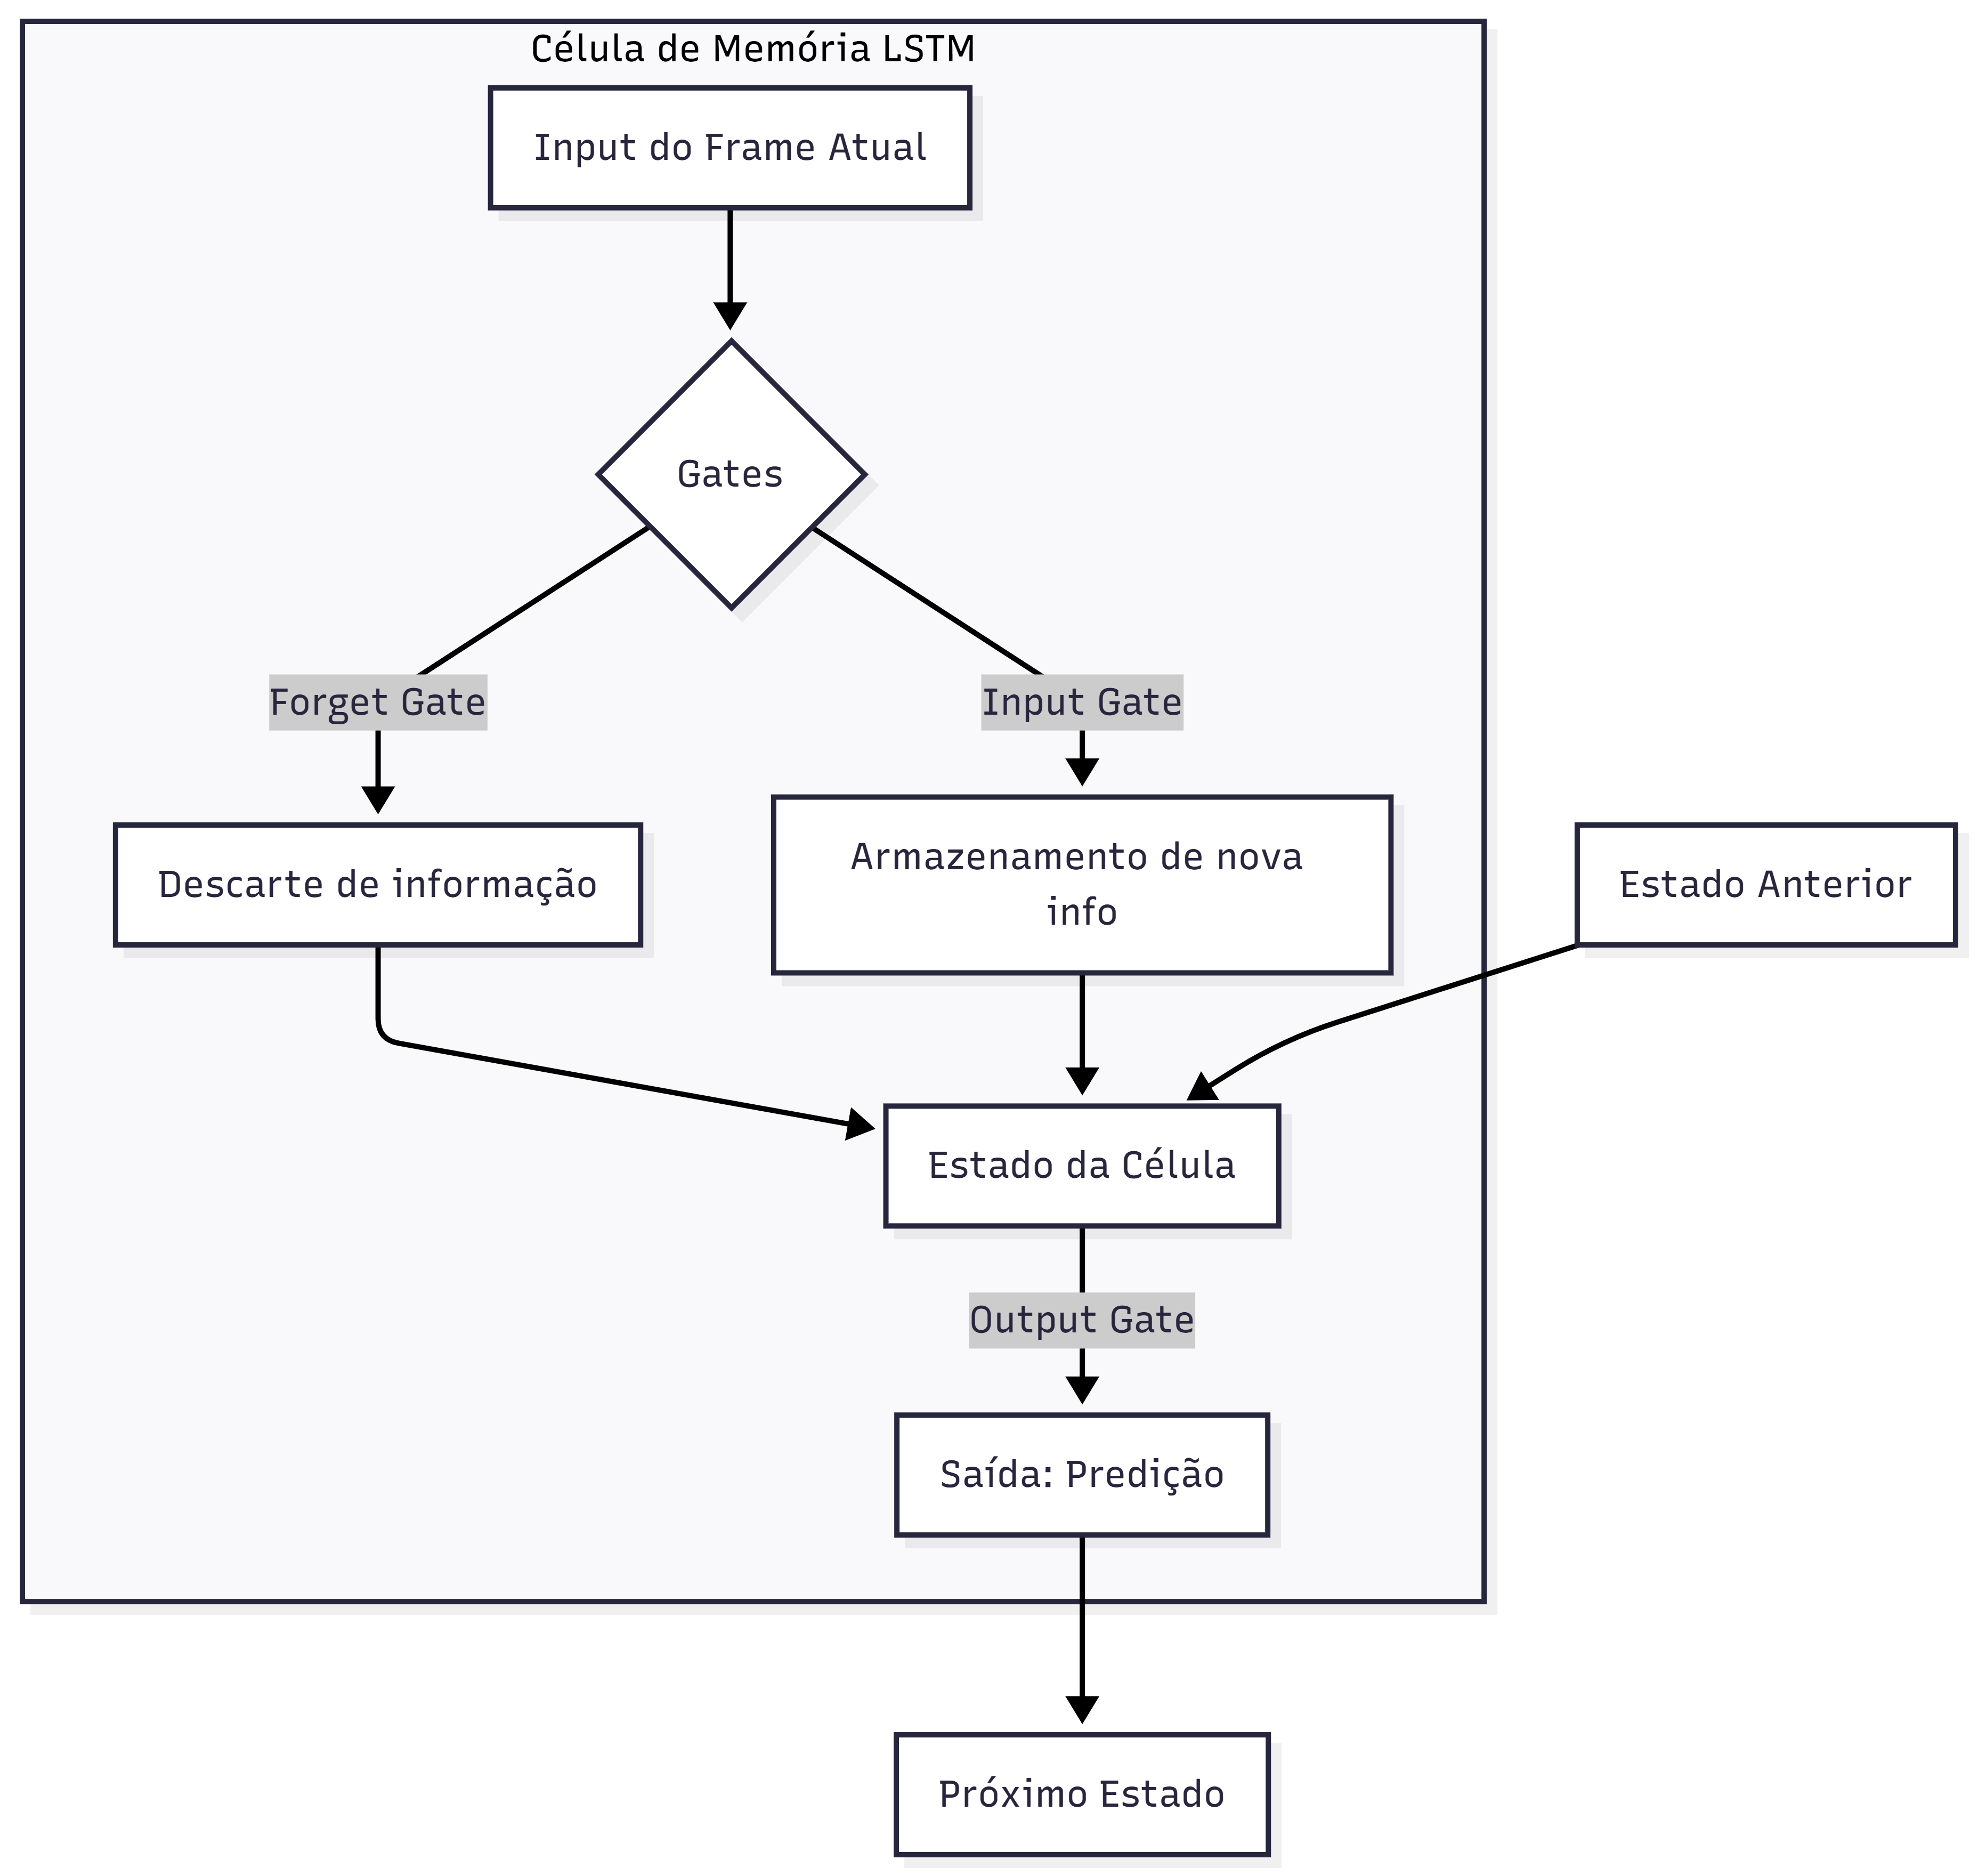
\includegraphics[width=0.8\textwidth]{./figuras/lstm}
    \caption{Diagrama de Rede Neural LSTM.}
    \label{fig:lstm}
    \source{Autoria própria (2026).}
\end{figure}

\begin{enumerate}
  \item Portão de Esquecimento (\textit{Forget Gate}): decide qual informação do estado anterior deve ser descartada;
  \item Portão de Entrada (\textit{Input Gate}): seleciona quais novas informações serão armazenadas no estado da célula;
  \item Portão de Saída (\textit{Output Gate}): determina qual parte do estado interno será enviada como saída para o próximo passo temporal (\cite{Contarini2020}; \cite{Almeida2019}).
\end{enumerate}

No contexto do tradutor de Libras, essa capacidade de retenção temporal permite que o sistema compreenda que a trajetória e a transição entre as poses das mãos são tão importantes quanto a configuração isolada em um único \textit{frame} \cite{Almeida2019}. Como destacado por \citeonline{Schmidhuber2014}, a profundidade dessas redes em termos de passos temporais possibilita a extração de representações abstratas que conectam movimentos manuais a conceitos semânticos complexos, garantindo maior precisão na interpretação de sinais dinâmicos.

\subsection{Reconhecimento de Gestos}

O reconhecimento de gestos é uma parte da visão computacional que visa identificar e interpretar movimentos ou posições do corpo humano a partir de dados visuais, transformando-os em comandos ou símbolos compreensíveis por máquinas \cite{Silva2017}. No contexto da Língua Brasileira de Sinais (Libras), essa técnica é o pilar fundamental para a tradução automatizada, permitindo que a interação entre surdos e ouvintes ocorra de forma fluida através da interface homem-máquina \cite{Bittencourt2002}.

Os gestos são geralmente classificados em duas categorias principais, cada uma exigindo abordagens algorítmicas distintas:
\begin{itemize}
    \item Estáticos (Imagem): Referem-se à configuração ou postura da mão em um único instante. O foco recai sobre a forma, a orientação e a posição dos dedos, como ocorre na representação do alfabeto manual ou numerais em Libras \cite{PintoJunior2019}. Redes Neurais Convolucionais (CNNs) são frequentemente aplicadas para extrair padrões espaciais nessas imagens estáticas.
    \item Dinâmicos (Vídeo): Envolvem uma sequência de movimentos ao longo do tempo, onde a trajetória e a velocidade são cruciais para o significado do sinal \cite{Silva2017}. Para interpretá-los, utilizam-se técnicas que consideram a continuidade temporal, como a subtração de quadros sucessivos para detecção de movimento ou o uso de grafos de ação e aprendizado de métricas para reconhecimento em tempo de execução \cite{Monteiro2016}.
\end{itemize}

A implementação eficaz desses sistemas enfrenta desafios significativos que podem comprometer a taxa de acerto do reconhecimento. As variações de iluminação representam um dos principais obstáculos, pois alterações na luz do ambiente modificam os valores dos pixels e dificultam a segmentação precisa da pele \cite{Bittencourt2002}. 

Além disso, a variabilidade entre usuários introduz complexidade, uma vez que diferentes pessoas possuem características físicas distintas e executam o mesmo sinal com velocidades e amplitudes diversas, exigindo modelos robustos e generalistas \cite{Silva2017}. 

Por fim, a influência do fundo da imagem (\textit{background}) pode impactar a precisão, especialmente em cenários com muitos objetos ou cores semelhantes ao tom da pele humana, o que torna essencial o uso de filtros adaptativos ou técnicas de segmentação para isolar adequadamente as mãos e o rosto do restante da cena \cite{Monteiro2016}.

\subsection{Processamento de Linguagem Natural}

O Processamento de Linguagem Natural é uma vertente da Inteligência Artificial que visa capacitar sistemas computacionais a compreender, interpretar e gerar a linguagem humana em formato de texto. Segundo \citeonline{Stryker2024}, o NLP combina a linguística estatística e computacional com modelos de \textit{deep learning} para processar a linguagem em formas que exibam compreensão de significado e intenção.

No escopo deste projeto, o reconhecimento isolado de gestos por meio de visão computacional não é suficiente para uma comunicação fluida, dada a profunda divergência gramatical entre a Libras e a língua portuguesa. Conforme apontam \citeonline{Lopez2017}, o uso de redes neurais aplicadas ao NLP permite que o sistema lide com a ambiguidade inerente à linguagem e aprenda representações hierárquicas dos dados textuais. O módulo de NLP atua, portanto, como uma camada de pós-processamento essencial, realizando a conversão semântica e sintática dos sinais identificados pela rede neural.

Antes de detalhar essa camada, é necessário esclarecer dois conceitos centrais utilizados ao longo desta e da próxima subseção: \textit{token} e \textit{pipeline}. Um \textit{token} é a menor unidade textual que um sistema de NLP manipula, obtida por meio da tokenização, processo que segmenta uma sentença em unidades discretas, como palavras, pontuações ou, no caso deste trabalho, sinais isolados reconhecidos pela visão computacional \cite{Bird2009}. Cada token é tratado individualmente pelas etapas seguintes do processamento, sendo posteriormente recombinado em uma estrutura gramatical coerente. 

Já um \textit{pipeline} é uma sequência ordenada de etapas de processamento, na qual a saída de uma etapa serve de entrada para a etapa seguinte \cite{Honnibal2020}. Essa organização em módulos encadeados permite decompor uma tarefa complexa, como transformar sinais soltos da Libras em uma frase gramaticalmente correta em português, em uma série de subtarefas menores, mais simples de implementar, testar e depurar de forma independente.

A ferramenta escolhida para implementar esse pipeline neste trabalho é a spaCy \cite{Honnibal2020}, uma biblioteca de código aberto para NLP escrita em Python e Cython. Diferentemente de bibliotecas voltadas majoritariamente para fins didáticos e experimentais, como o NLTK, a spaCy foi projetada com foco industrial (\textit{industrial-strength}), priorizando desempenho, eficiência de memória e facilidade de uso em aplicações de produção \cite{Honnibal2020}.

Um dos principais diferenciais da spaCy é justamente sua organização nativa em pipelines pré-configurados: ao carregar um modelo de linguagem treinado, o texto de entrada é processado automaticamente por uma sequência integrada de componentes, entre eles o tokenizador, o \textit{tagger} morfossintático, o analisador de dependências sintáticas e um reconhecedor de entidades nomeadas (NER), sem que seja necessário implementar cada uma dessas etapas manualmente \cite{Honnibal2020}. Internamente, a biblioteca representa o resultado desse processamento por meio de objetos como \texttt{Doc} (o texto processado como um todo), \texttt{Token} (cada unidade individual) e \texttt{Span} (trechos contínuos de tokens), o que facilita a navegação programática pelas relações identificadas em cada sentença.

Além dos componentes padrão, a spaCy permite estender ou substituir qualquer etapa do pipeline por meio de componentes customizados, inseridos com o método \texttt{nlp.add\_pipe} \cite{Honnibal2020}. É essa extensibilidade que viabiliza acoplar o próprio módulo de reordenação sintática, como uma etapa adicional do pipeline, executada logo após a análise de dependências nativa da biblioteca. Para a etiquetagem e a análise sintática em português, a spaCy disponibiliza pipelines pré-treinados específicos para o idioma, como o \texttt{pt\_core\_news\_sm}, o \texttt{pt\_core\_news\_md} e o \texttt{pt\_core\_news\_lg}, que se diferenciam entre si pelo tamanho do vocabulário e pela presença de vetores de palavras, impactando diretamente a acurácia da etiquetagem e da análise de dependências \cite{Honnibal2020}.

Na abordagem adotada neste trabalho, esse pipeline é composto por 5 etapas fundamentais, ilustradas no diagrama da Figura \ref{fig:pipeline_nlp}: tokenização e normalização, etiquetagem morfossintática, análise de dependência sintática e, por fim, reordenação sintática e concordância.

\begin{figure}[H]
    \centering
    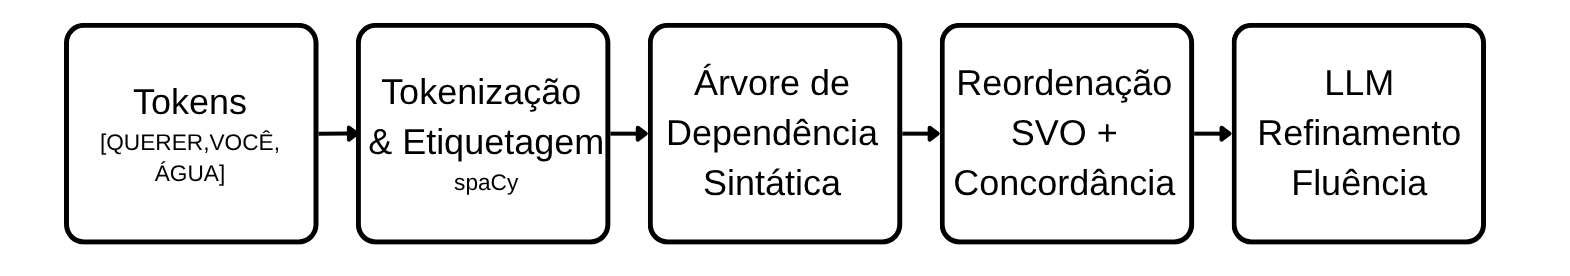
\includegraphics[width=1.0\textwidth]{./figuras/processamento-de-imagem-nlp}
    \caption{Diagrama de Processamento de Linguagem Natural - NLP.}
    \label{fig:pipeline_nlp}
    \source{Autoria própria (2026).}
\end{figure}

Os sinais identificados pela etapa de visão computacional chegam ao módulo de NLP como uma sequência de \textit{tokens}, palavras isoladas na estrutura da Libras (ex.: \texttt{[VOCÊ, QUERER, ÁGUA]}). A tokenização consiste em tratar cada sinal como uma unidade lexical discreta, e a normalização realiza a lematização de cada token, reduzindo as formas flexionadas à forma canônica (lema), o que facilita o mapeamento para o português \cite{Bird2009}.

Cada token recebe uma etiqueta morfossintática (substantivo, verbo, pronome, etc.). No spaCy, esse processo é realizado por um modelo de rede neural treinado sobre corpora anotados \cite{Honnibal2020}. Formalmente, dado um vocabulário $\mathcal{V}$ e um conjunto de etiquetas $\mathcal{T}$, o \textit{tagger} aprende uma função $f: \mathcal{V}^n \rightarrow \mathcal{T}^n$ que maximiza a probabilidade conjunta da sequência de etiquetas dado o contexto da sentença.

Após a etiquetagem, o analisador de dependências identifica as relações gramaticais entre os tokens (sujeito, objeto, modificador, etc.), produzindo uma árvore de dependência sintática.

Com base nas relações identificadas pela árvore de dependência, o módulo reordena os tokens segundo a estrutura SVO do português e aplica regras de concordância nominal e verbal. Por exemplo, a sequência da Libras \texttt{[VOCÊ, QUERER, ÁGUA]} é reescrita como \textit{``Você quer água.''}, com a flexão verbal adequada ao sujeito identificado \cite{Lopez2017}.

Formalmente, seja $S_L = (w_1, w_2, \ldots, w_n)$ a sequência de sinais identificados na estrutura da Libras e $S_P$ a frase-alvo em português. O módulo de NLP aprende uma função de reordenação $\pi$ tal que: 

\begin{equation}
    S_P = \text{Flexão}\bigl(\pi(S_L),\; G_{\text{pt}}\bigr)
\end{equation}

onde $\pi$ é uma permutação dos índices dos tokens guiada pelas relações de dependência e $G_{\text{pt}}$ representa as regras gramaticais do português, incluindo concordância de gênero, número e tempo verbal \cite{Bird2009}.

\subsection{Árvores de Dependência Sintática}

Uma árvore de dependência sintática é uma estrutura de dados que representa as relações gramaticais binárias e assimétricas entre os tokens de uma sentença. Diferentemente das gramáticas de constituintes (baseadas em sintagmas), a análise de dependência conecta diretamente pares de palavras: uma cabeça e um dependente, com uma etiqueta que nomeia o tipo de relação (\textit{nsubj} para sujeito nominal, \textit{obj} para objeto direto, \textit{advmod} para modificador adverbial, etc.) \cite{Jurafsky2023}.

Formalmente, dada uma sentença $s = (w_1, w_2, \ldots, w_n)$, uma árvore de dependência é um grafo dirigido $G = (V, A)$ onde:

\begin{itemize}
    \item $V = \{w_0, w_1, \ldots, w_n\}$ é o conjunto de vértices (tokens mais um nó raiz artificial $w_0$);
    \item $A \subseteq V \times V \times \mathcal{R}$ é o conjunto de arcos rotulados, onde cada arco $(w_i, w_j, r)$ indica que $w_i$ é a cabeça de $w_j$ com relação do tipo $r \in \mathcal{R}$;
    \item cada token (exceto a raiz) possui exatamente uma cabeça, garantindo a estrutura de árvore \cite{Jurafsky2023}.
\end{itemize}

Como exemplo, considere a sentença \textit{``Você quer água.''} Sua árvore de dependência teria \textit{quer} como raiz (verbo principal), com \textit{Você} ligado a ela pelo arco \texttt{nsubj} (sujeito nominal) e \textit{água} pelo arco \texttt{obj} (objeto direto), conforme exemplificado na estrutura da Figura \ref{fig:arvore_dependencia}.

\begin{figure}[H]
    \centering
    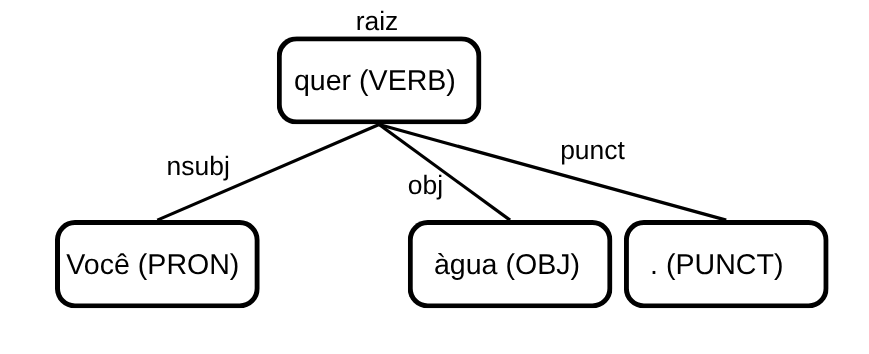
\includegraphics[width=0.7\textwidth]{./figuras/arvoreDependencia.png}
    \caption{Exemplo estrutural de uma árvore de análise por dependência sintática.}
    \label{fig:arvore_dependencia}
    \source{Autoria própria (2026).}
\end{figure}

No presente trabalho, a análise de dependência é realizada pela biblioteca spaCy \cite{Honnibal2020}, que implementa um analisador neural baseado em transições (\textit{transition-based parser}). Esse analisador processa a sentença da esquerda para a direita, mantendo uma pilha e uma fila de tokens, e a cada passo aplica uma das três operações possíveis: \textit{SHIFT} (empilha o próximo token), \textit{LEFT-ARC} (cria um arco da cabeça para o dependente à esquerda) ou \textit{RIGHT-ARC} (cria um arco da cabeça para o dependente à direita). A escolha da operação é feita por um classificador neural que considera o contexto da pilha e da fila \cite{Honnibal2020}.

A adoção de árvores de dependência é especialmente adequada para este projeto por três razões. Primeiro, como a Libras apresenta ordem frasal flexível (SVO, SOV, OSV, entre outras), a análise de dependência é robusta a variações de ordem, pois identifica as relações semânticas independentemente da posição linear dos tokens \cite{Jurafsky2023}. Segundo, a estrutura arbórea explicita quais tokens são sujeito, objeto e predicado, fornecendo ao módulo de reordenação a informação necessária para reconstruir a sentença na estrutura SVO do português. Terceiro, as etiquetas de dependência permitem aplicar regras de concordância dirigidas: identificado o sujeito (\texttt{nsubj}), é possível flexionar o verbo-cabeça no número e pessoa correspondentes \cite{Bird2009}.

Dessa forma, as árvores de dependência atuam como a representação intermediária que conecta a saída do reconhecedor de gestos (sequência de tokens na ordem da Libras) à frase final gramaticalmente correta em português, tornando o pipeline de tradução mais explícito, interpretável e extensível.

\subsection{Modelos de Linguagem de Grande Escala}

Os Modelos de Linguagem de Grande Escala (LLMs, do inglês \textit{Large Language Models}) são sistemas de inteligência artificial treinados em vastos volumes de dados, especializados na compreensão e geração de texto com alta fluência. 

Diferente das arquiteturas de \textit{deep learning} voltadas para o processamento de sequências de dados brutos, os LLMs baseiam-se na arquitetura Transformer \cite{Vaswani2017}, cujo mecanismo de \textit{self-attention} permite ao modelo ponderar a relevância de todos os tokens de uma sentença simultaneamente, capturando dependências contextuais de longo alcance com maior eficiência do que arquiteturas recorrentes como a LSTM.

No fluxo de tradução proposto, o LLM atua como uma camada de refinamento linguístico final. Após o módulo de NLP (spaCy) organizar a estrutura sintática básica e realizar as flexões necessárias, o LLM recebe essa sentença intermediária para otimizar sua naturalidade. Essa etapa é essencial para ajustar nuances que as regras gramaticais rígidas podem não captar, como a inserção de conectivos contextuais ou o ajuste de registro (formal ou informal), garantindo que a saída em português não seja apenas gramaticalmente correta, mas também fluida para o ouvinte.

A integração de modelos como \textit{Llama} \cite{Touvron2023} ou \textit{Gemma} \cite{GemmaTeam2024} permite que o sistema aproveite a capacidade de \textit{few-shot learning} \cite{Brown2020}, ou seja, a habilidade do modelo em refinar traduções a partir de poucos exemplos de contexto, sem a necessidade de um novo treinamento exaustivo. Assim, o projeto estabelece uma arquitetura híbrida e colaborativa.

\subsection{Custo Computacional e Peso dos Modelos}

O custo computacional refere-se à quantidade de recursos necessários para executar um modelo, incluindo uso de memória, processamento e capacidade de armazenamento. Já o peso do modelo está relacionado ao número de parâmetros treináveis presentes na rede neural, influenciando diretamente seu tamanho e complexidade.

Modelos mais complexos, como redes profundas com múltiplas camadas, tendem a apresentar maior precisão, porém demandam mais recursos computacionais. Conforme discutido por \citeonline{Goodfellow2016}, o aumento da profundidade das redes neurais eleva sua capacidade de representação, mas também implica maior custo de processamento e necessidade de hardware mais robusto.

No contexto deste trabalho, a escolha das arquiteturas busca equilibrar desempenho e eficiência, considerando a necessidade de processamento em tempo execução. Estratégias como o uso de \textit{landmarks}, redução de dimensionalidade dos dados e limitação do vocabulário contribuem para diminuir o custo computacional.

Esse equilíbrio é fundamental para garantir que o sistema seja não apenas preciso, mas também utilizável em cenários práticos.

\subsection{Acurácia \& Precisão}

A acurácia é uma métrica que expressa a proporção de predições corretas em relação ao total de exemplos avaliados, oferecendo uma visão geral do desempenho do sistema \cite{Goodfellow2016}. Apesar de sua interpretação direta, a acurácia isolada pode ser insuficiente em contextos com muitas classes, pois não revela quais sinais estão sendo confundidos entre si, informação essencial para o refinamento do modelo.

Para suprir essa limitação, utiliza-se a matriz de confusão, uma representação tabular que cruza as classes reais com as classes preditas. Cada célula indica quantas amostras de uma determinada classe foram classificadas como outra, permitindo identificar padrões de erro específicos. Por exemplo, quais pares de sinais o modelo tende a confundir com maior frequência devido à semelhança na configuração de mão ou no movimento \cite{Goodfellow2016}. A partir dela, derivam-se ainda métricas complementares como precisão e \textit{recall}, que expõem desequilíbrios de desempenho entre as classes de forma mais granular.

A estrutura básica de uma matriz de confusão pode ser observada na Figura \ref{fig:matriz_confusao}. Nela, os resultados de classificação são organizados em verdadeiros positivos (VP), verdadeiros negativos (VN), falsos positivos (FP) e falsos negativos (FN), permitindo uma análise detalhada dos acertos e erros cometidos pelo modelo durante o processo de classificação.

\begin{figure}[H]
    \centering
    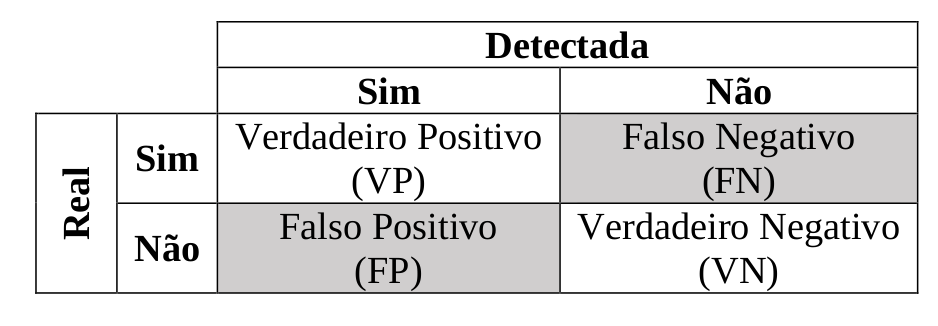
\includegraphics[width=0.7\textwidth]{./figuras/matrizConfusao.png}
    \caption{Estrutura conceitual de uma matriz de confusão.}
    \label{fig:matriz_confusao}
    \noindent\footnotesize{Fonte: Adaptado de \citeonline{Nogare2020}.}
\end{figure}

No escopo desta pesquisa, a acurácia e a matriz de confusão serão utilizadas para avaliar o módulo de visão computacional, tanto na classificação de sinais estáticos pela CNN quanto no reconhecimento de sinais dinâmicos pela LSTM. A análise conjunta dessas métricas permitirá identificar os sinais com maior taxa de erro e orientar ajustes no modelo ou na composição do \textit{dataset} de treinamento.

Com essa abordagem, busca-se garantir que o sistema apresente desempenho equilibrado entre todos os sinais do vocabulário definido, e não apenas nas classes mais frequentes.

\subsection{Métrica BLEU}

A métrica BLEU (\textit{Bilingual Evaluation Understudy}), proposta por \citeonline{Papineni2002}, é o padrão consolidado para avaliação automática de qualidade em sistemas de tradução. Ela compara o texto gerado pelo sistema com traduções humanas de referência, mensurando a sobreposição de sequências de palavras conhecidas como $n$-gramas. Esses elementos representam agrupamentos contínuos de $n$ itens; enquanto os unigramas ($n=1$) avaliam a presença de palavras isoladas, os bigramas ($n=2$) e trigramas ($n=3$) permitem verificar se a ordem e o contexto gramatical foram preservados. Quanto maior a correspondência com as referências humanas, mais alto o escore BLEU, que varia de 0 a 1.

O uso do BLEU é especialmente relevante neste projeto porque o pipeline de pós-processamento, que integra o módulo de NLP e o refinamento via LLM, não apenas transcreve sinais isolados, mas reorganiza, flexiona e contextualiza as palavras para gerar frases fluidas em português, um processo que não pode ser avaliado somente por métricas de classificação tradicionais \cite{Vaswani2017, Touvron2023}. Conforme apontam \citeonline{Papineni2002}, a métrica captura tanto a precisão lexical quanto aspectos da fluência, ao penalizar hipóteses que se distanciam estruturalmente das referências humanas.

Para a validação do sistema proposto, o BLEU será calculado comparando as sentenças finais em português (após o refinamento linguístico realizado pelo LLM) com traduções de referência elaboradas por intérpretes de Libras para o mesmo conjunto de sinais de entrada \cite{Touvron2023}. Escores mais altos indicam que a integração entre NLP e LLM é capaz de gerar saídas linguisticamente próximas ao que um humano produziria a partir dos mesmos sinais \cite{Touvron2023}.

Nesse sentido, o BLEU complementa as métricas de reconhecimento gestual ao avaliar especificamente a qualidade da camada linguística do sistema, fechando o ciclo de avaliação do pipeline completo de tradução.

\subsection{Latência e Tempo de Resposta}

A latência corresponde ao tempo decorrido entre a captura do sinal pelo sistema e a exibição da tradução ao usuário. Em aplicações de tradução em tempo real, esse fator é crítico, pois impacta diretamente a experiência de uso e a fluidez da comunicação.

Sistemas com alta latência podem gerar atrasos perceptíveis, comprometendo a interação entre os usuários. Por isso, é necessário otimizar todas as etapas do pipeline, desde a captura do vídeo até o processamento pelos modelos e a geração da saída textual.

De acordo com \citeonline{Molchanov2015}, em sistemas de reconhecimento de gestos em tempo real, o desempenho está diretamente relacionado à eficiência computacional dos modelos e à capacidade de processar sequências de vídeo com baixa latência.

No presente trabalho, a latência será considerada como um dos principais critérios de avaliação do sistema. A utilização de técnicas como processamento eficiente de \textit{frames}, redução do tamanho dos dados (por meio de \textit{landmarks}) e escolha de modelos com menor custo computacional contribui para minimizar o tempo de resposta.

Dessa forma, busca-se garantir que a tradução ocorra de forma rápida e contínua, aproximando-se de uma comunicação natural.

% ---------------------------------------------------------------
\section{Trabalhos correlatos}
\label{sec:trabalhos_correlatos}

\subsection{Trabalho 1: Sign Language Translator System Using Computer Vision and LSTM Neural Networks}

O estudo de \citeonline{Wang2025} investigou o problema da dificuldade de comunicação entre pessoas surdas e ouvintes, causada pela falta de compreensão da língua de sinais, o que impacta diretamente o acesso a serviços e interações sociais, o mesmo problema abordado neste trabalho.

Para enfrentar essa questão, os autores desenvolveram um sistema de tradução de língua de sinais em tempo real, combinando técnicas de visão computacional, redes neurais convolucionais (CNN), redes recorrentes do tipo LSTM e processamento de linguagem natural. A metodologia incluiu a coleta e anotação de um \textit{dataset} de gestos, seguido do treinamento de modelos capazes de reconhecer sinais e convertê-los em texto automaticamente.

Os resultados obtidos demonstraram uma precisão de 97\% no reconhecimento dos gestos, indicando que a abordagem é eficaz para cenários controlados. Além disso, o sistema mostrou potencial para melhorar a acessibilidade e a inclusão social.

Entretanto, a solução apresenta limitações importantes, como a dependência de condições ambientais controladas (iluminação e fundo), a escassez de \textit{datasets} amplos, e dificuldades em manter desempenho em tempo real. Também há restrições relacionadas à acessibilidade, especialmente em sistemas baseados na web que dependem de conexão com a internet.

Diferentemente desse trabalho, a presente pesquisa propõe uma abordagem mais integrada, ao não apenas reconhecer os sinais, mas também estruturá-los linguisticamente por meio de processamento de linguagem natural, buscando gerar frases coerentes em português, e não apenas transcrições diretas de sinais.

\subsection{Trabalho 2: Interpretação de gestos de Libras usando K-Means e Random Forest}

\citeonline{Caiafa2023} propuseram uma solução para o reconhecimento automático de sinais da Libras com foco em reduzir o custo computacional, mantendo uma boa acurácia. O problema tratado também está relacionado à barreira de comunicação entre usuários e não usuários da língua de sinais, sendo, portanto, diretamente alinhado com esta pesquisa.

A abordagem adotada pelos autores difere das soluções baseadas exclusivamente em \textit{deep learning}, pois utiliza o MediaPipe para extração de pontos-chave corporais, seguido de técnicas de agrupamento com K-Means e classificação utilizando algoritmos como KNN e Random Forest. Essa metodologia permite trabalhar com representações mais leves dos dados, reduzindo o processamento necessário.

Os experimentos foram realizados utilizando a \textit{dataset} MINDS-Libras, resultando em uma acurácia de 94,72\%, demonstrando que a solução é eficiente mesmo com menor complexidade computacional.

Apesar dos bons resultados, o trabalho apresenta limitações, principalmente no fato de que o sistema foca apenas na classificação de sinais isolados, sem tratar a construção de frases ou o contexto linguístico. Além disso, ainda enfrenta desafios comuns da área, como variações de iluminação, ângulo de câmera e aumento do vocabulário.

O presente trabalho avança em relação a essa proposta ao incorporar, além da etapa de reconhecimento, um módulo de processamento de linguagem natural, responsável por organizar os sinais identificados em frases estruturadas em português, ampliando o nível de interpretação da comunicação.

\subsection{Trabalho 3: Detection and Interpretation of Indian Sign Language Using LSTM Networks}

\citeonline{Vyavahare2023} abordaram o desenvolvimento de um sistema para reconhecimento e interpretação da língua de sinais indiana (ISL) em tempo real, com o objetivo de reduzir a lacuna comunicacional entre pessoas com deficiência auditiva e a sociedade, problema equivalente ao tratado neste TCC.

A solução proposta baseia-se no uso de técnicas de visão computacional para extração de características visuais, combinadas com redes neurais recorrentes do tipo LSTM, capazes de capturar dependências temporais em gestos dinâmicos. Os autores também criaram um \textit{dataset} próprio, composto por vídeos anotados de usuários nativos de ISL.

Os resultados experimentais indicaram um desempenho elevado, com 96\% de acurácia no treinamento e 87\% no teste, evidenciando a capacidade do modelo em reconhecer padrões gestuais dinâmicos.

No entanto, o estudo apresenta algumas limitações relevantes. A principal delas é que o sistema está restrito ao reconhecimento de palavras isoladas, não sendo capaz de interpretar frases completas. Além disso, o desempenho pode ser afetado por fatores como variações de iluminação, ângulo de câmera e posicionamento das mãos.

Este trabalho propõe uma solução que vai além do reconhecimento de gestos individuais, incorporando uma camada de processamento de linguagem natural para construção de frases, buscando uma tradução mais próxima da comunicação real entre Libras e língua portuguesa.

\vspace{0.5cm}

\begin{table}[htb]
    \centering
    \caption{Comparação entre trabalhos relacionados}
    \label{tab:trabalhos_relacionados}
    \small % Reduz levemente o tamanho da fonte para caber melhor na página
    \begin{tabular}{p{2cm}|p{3cm}|p{3cm}|p{3cm}|p{3cm}}
        \toprule
        \textbf{Critério} & \textbf{Trabalho 1} & \textbf{Trabalho 2} & \textbf{Trabalho 3} & \textbf{Este trabalho} \\
        \midrule
        \textbf{Objetivo} 
        & Tradução de sinais em tempo real para texto. 
        & Classificação de sinais de Libras com baixo custo computacional. 
        & Reconhecimento e interpretação de sinais dinâmicos (ISL). 
        & Tradução de Libras com estruturação gramatical de frases. \\
        \midrule
        \textbf{Tecnologia} 
        & CNN, LSTM e NLP básico. 
        & MediaPipe, K-Means, KNN e Random Forest. 
        & Visão Computacional (OpenCV) e LSTM. 
        & Arquitetura híbrida CNN + LSTM e camada robusta de NLP. \\
        \midrule
        \textbf{Validação} 
        & Dataset próprio (webcam); Acurácia de 97\%. 
        & Base pública MINDS-Libras; Acurácia de 94,72\%. 
        & Dataset próprio (ISL); 96\% treino e 87\% teste. 
        & Dataset de Libras, métricas de acurácia e avaliação sintática. \\
        \midrule
        \textbf{Limitação} 
        & Sensível à iluminação e dependência de conexão web. 
        & Classificação restrita a sinais/palavras isoladas. 
        & Não interpreta frases completas ou contexto linguístico. 
        & Dependência de \textit{dataset} abrangente para diversidade de sinais. \\
        \bottomrule
    \end{tabular}
    \\
    \source{Autoria própria (2026).}
\end{table}

% ===============================================================
% CAPÍTULO 3 - DESENVOLVIMENTO
% ===============================================================
\chapter{Desenvolvimento / Implementação / Experimentos}
\label{cap:desenvolvimento}

% ---------------------------------------------------------------
\section{Metodologia da pesquisa}
\label{sec:metodologia_pesquisa}

Descreva, de forma rigorosa e reprodutível, como a pesquisa foi conduzida. Informe o tipo de pesquisa (exploratória, empírica, formal etc.) e a hipótese ou o critério de sucesso adotado; detalhe os procedimentos da abordagem proposta, em ordem cronológica (use listas numeradas, diagramas de fluxo ou pseudocódigo para tornar o processo claro); liste as ferramentas, linguagens, bibliotecas, frameworks e ambientes utilizados, justificando cada escolha com base no problema; e explique como os experimentos foram configurados, quais variáveis foram controladas e quais métricas demonstram que a proposta cumpre os objetivos (ex.: acurácia, latência, custo).

\begin{table}[htb]
  \centering
  \caption{Plano de experimentação}
  \label{tab:plano_experimentos}
  \begin{tabular}{lcc}
    \toprule
    \textbf{Experimento} & \textbf{Variável controlada} & \textbf{Métrica principal} \\
    \midrule
    Comparação com baseline & algoritmo & acurácia \\
    Escalabilidade & carga & tempo médio \\
    \bottomrule
  \end{tabular}
  \legend{Fonte: Elaborado pelo autor (2025)}
\end{table}

\textit{Propor algo não basta: demonstre como será validado.}

\section{Detalhes da implementação}
\label{sec:implementacao}

Explique a modelagem e a arquitetura da solução (diagramas UML, blocos ou fluxogramas que mostrem como os módulos se relacionam e atendem ao problema), as escolhas tecnológicas, as estruturas de dados e as integrações. Quando esclarecerem decisões de pesquisa, inclua trechos de código relevantes ou pseudoexemplos. Caso o trabalho envolva dados, descreva também como eles foram coletados (logs, sensores, APIs), armazenados e preparados (limpeza, normalização, anonimização).

% ---------------------------------------------------------------
% EXEMPLO DE INSERÇÃO DE FIGURA (substitua pela sua imagem)
% A imagem deve ficar na pasta assets/ (ex.: assets/figures/arquitetura.png).
% ORDEM ABNT: o título (\caption) vem ACIMA da figura e a fonte
% (\legend) vem ABAIXO. Por isso \caption e \label aparecem ANTES do
% \includegraphics. Use \ref{...} para citar a figura no texto.
% ---------------------------------------------------------------
\begin{figure}[htb]
    \centering
    \caption{Exemplo de inserção de figura --- substitua pelo diagrama da arquitetura da sua solução.}
    \label{fig:arquitetura}
    \includegraphics[width=0.35\textwidth]{assets/logo-senac.png}
    \legend{Fonte: Elaborado pelo autor (2025)}
\end{figure}

Toda figura deve ser numerada, ter legenda (\verb|\caption|) e indicação de fonte, além de ser citada no texto --- por exemplo, a Figura~\ref{fig:arquitetura}. As figuras com legenda aparecem automaticamente na \textit{Lista de ilustrações}, nos elementos pré-textuais.

\section{Experimentos e cenário de testes (opcional)}
\label{sec:experimentos}

Esta seção é \textbf{opcional} e deve ser incluída quando o trabalho prevê avaliação experimental. Descreva os cenários planejados, os parâmetros testados e por que cada experimento está alinhado aos objetivos. Liste os conjuntos de dados, as variações e o número de repetições.

\section{Resultados e análises}
\label{sec:resultados}

Apresente os resultados com tabelas, gráficos e figuras e, sobretudo, \textbf{analise-os} à luz da revisão bibliográfica e da hipótese --- resultados devem ser analisados, não apenas exibidos. Diferencie:
\begin{itemize}
  \item \textbf{Figura:} imagens, diagramas conceituais ou arquiteturais que ilustram estrutura ou fluxo.
  \item \textbf{Gráfico:} plot de dados (linhas, barras, boxplots) que compara métricas obtidas.
\end{itemize}

Exemplo de tabela:
\begin{table}[htb]
  \centering
  \caption{Comparação de métricas reportadas}
  \label{tab:metricas}
  \begin{tabular}{lcc}
    \toprule
    Método & Acurácia & Tempo médio (ms) \\
    \midrule
    Proposta & 92\% & 180 \\
    Baseline & 88\% & 220 \\
    \bottomrule
  \end{tabular}
  \legend{Fonte: Elaborado pelo autor (2025)}
\end{table}

Ao inserir um gráfico (por exemplo \texttt{assets/figures/desempenho.png}), use --- lembrando que, pela ABNT, o \texttt{\textbackslash caption} (título) vem \textbf{acima} da imagem e a fonte (\texttt{\textbackslash legend}) vem \textbf{abaixo}:
\begin{verbatim}
\begin{figure}[htb]
  \centering
  \caption{Gráfico de comparação das métricas de acurácia.}
  \label{fig:grafico-desempenho}
  \includegraphics[width=0.8\textwidth]{assets/figures/desempenho.png}
  \legend{Fonte: Elaborado pelo autor (2025)}
\end{figure}
\end{verbatim}

Na sequência, faça a \textbf{análise crítica e comparação}, discutindo as descobertas em relação aos trabalhos correlatos e evidenciando ganhos e perdas; por fim, na \textbf{discussão}, relacione os resultados aos objetivos e à hipótese, explicitando se o critério de sucesso foi atingido.

\textit{O desenvolvimento só é pesquisa se estiver claramente ligado ao problema e à metodologia definida.}

% ---------------------------------------------------------------
% CONCLUSÃO
% ---------------------------------------------------------------
\chapter{Conclusão}

\section{Retomada do problema e dos objetivos}
Retome o problema e destaque o que foi atingido.

\section{Contribuições para a Computação}
Explique o que a pesquisa trouxe de novo.

\section{Limitações e trabalhos futuros}
Liste limites e sugira próximos passos coerentes.

% ---------------------------------------------------------------
% OBSERVAÇÕES DO AUTOR
% ---------------------------------------------------------------
\chapter*{Observações importantes}
\addcontentsline{toc}{chapter}{Observações importantes}

Para graduação, Wazlawick aceita trabalhos aplicados desde que:
\begin{itemize}
    \item O problema seja preciso;
    \item A solução esteja fundamentada;
    \item Haja análise crítica;
    \item Não seja apenas entrega funcional.
\end{itemize}

% ---------------------------------------------------------------
% APRESENTAÇÃO ORAL (BANCA)
% ---------------------------------------------------------------
\chapter*{Apresentação oral (banca)}
\addcontentsline{toc}{chapter}{Apresentação oral (banca)}

Além do documento escrito, o TCC2 é avaliado por uma \textbf{apresentação oral} final perante a banca. Um template pronto em \texttt{Beamer} está disponível no arquivo \texttt{apresentacao\_tcc2.tex}, na mesma pasta deste documento.

\noindent\fbox{\parbox{\dimexpr\textwidth-2\fboxsep-2\fboxrule}{%
\textbf{Regras da apresentação do TCC2}

\vspace{0.2cm}
\begin{itemize}
    \item \textbf{Duração: 30 minutos.} Cronometre os ensaios; ultrapassar o tempo é penalizado. A arguição da banca ($\approx$ 5 min) ocorre após a apresentação, separada desse total.
    \item \textbf{Cubra o trabalho completo}, seguindo a estrutura do documento escrito: introdução e problema, objetivos e método, desenvolvimento, \textbf{resultados e análise} e conclusão/contribuições.
    \item \textbf{Dê peso aos resultados:} grande parte do tempo deve ser dedicada a apresentar e \textbf{analisar criticamente} os resultados, não apenas descrevê-los.
    \item \textbf{Ritmo:} cerca de 1 a 1,5 minuto por slide, totalizando aproximadamente 20 a 26 slides de conteúdo.
    \item \textbf{Logo do SENAC:} grande no primeiro slide (capa) e pequena no canto superior direito dos demais slides --- já configurado no template.
    \item \textbf{Demonstração:} se houver demo ao vivo, tenha um plano B com capturas de tela ou vídeo curto.
    \item \textbf{Slides de apoio (backup):} inclua slides extras após o ``Obrigado'' com detalhes técnicos, trechos de código e tabelas completas para a arguição.
\end{itemize}

\vspace{0.2cm}
\textbf{Distribuição de tempo sugerida (30 min):} introdução/problema $\approx$ 4 min; objetivos/método $\approx$ 5 min; desenvolvimento $\approx$ 8 min; resultados/análise $\approx$ 8 min; conclusão $\approx$ 3 min; demonstração $\approx$ 2 min.
}}

% ---------------------------------------------------------------
% ELEMENTOS PÓS-TEXTUAIS
% ---------------------------------------------------------------
\postextual

% ===============================================================
% REFERÊNCIAS BIBLIOGRÁFICAS
% ===============================================================
% As referências bibliográficas são geradas automaticamente a partir
% do arquivo bibliografia_tcc2.bib, seguindo o padrão ABNT (NBR 6023).
%
% COMO CITAR no texto:
%   \cite{chave}         -> (SOBRENOME, ano) — citação indireta
%   \citeonline{chave}   -> Sobrenome (ano) — citação direta no texto
%
% TIPOS DE REFERÊNCIA no arquivo .bib:
%   @book        -> Livros
%   @article     -> Artigos de periódicos
%   @inproceedings -> Artigos em anais de eventos
%   @mastersthesis -> Dissertações de mestrado
%   @phdthesis   -> Teses de doutorado
%   @misc        -> Sites, vídeos e outros materiais
%   @manual      -> Documentação técnica
% ---------------------------------------------------------------
\bibliography{bibliografia_tcc2}

% ---------------------------------------------------------------
% APÊNDICES (se necessário)
% ---------------------------------------------------------------
% \begin{apendicesenv}
% \partapendices
%
% \chapter{Nome do Apêndice}
% \label{ap:apendice1}
%
% Conteúdo do apêndice (material elaborado pelo próprio autor).
%
% \end{apendicesenv}

% ---------------------------------------------------------------
% ANEXOS (se necessário)
% ---------------------------------------------------------------
% \begin{anexosenv}
% \partanexos
%
% \chapter{Nome do Anexo}
% \label{an:anexo1}
%
% Conteúdo do anexo (material de terceiros).
%
% \end{anexosenv}

\end{document}
